\chapter{HIỆN THỰC VÀ THỬ NGHIỆM}

% **************************** Define Graphics Path **************************
\ifpdf
    \graphicspath{{Chapter3/Figs/Raster/}{Chapter3/Figs/server/}{Chapter3/Figs/}}
\else
    \graphicspath{{Chapter3/Figs/Vector/}{Chapter3/Figs/}}
\fi

\section{Hiện thực node cảm biến}
\subsection{Hiện thực prototype node cảm biến}
Chức năng chính của node cảm biến là dùng để lấy các dữ liệu môi trường như giá trị nồng độ CO, chất lượng không khí, nhiệt độ và lượng bụi, trong quá trình tìm các loại cảm biến trên thị trường hiện có thì nhóm chúng tôi đã đề xuất sử dụng các cảm biến được đề cập tại mục \ref{sec:cacloaicambien} như sau:
\begin{itemize}
	\item[•]Cảm biến GP2: dùng để đo lượng bụi có trong không khí.
	\item[•]Cảm  biến MQ135: dùng để đo chất lượng của môi trường không khí.
	\item[•]Cảm biến MQ07: dùng để đo nồng độ khí CO trong không khí.
	\item[•]Cảm biến DS18B20: dùng để đo nhiệt độ môi trường xung quanh. 
\end{itemize}
Như vậy, các thành phần chính của prototype biến đầu tiên chúng tôi đã xây dựng như sau:
\begin{figure}[H]
	\centering    
	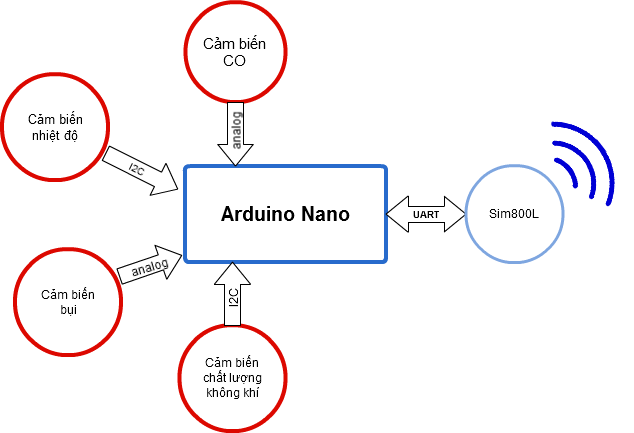
\includegraphics[width=5in]{prototype_1}
	\caption[Mô hình prototype đầu tiên]{Mô hình prototype đầu tiên}
	\label{fig:prototype_1}
\end{figure}
Ngoài những cảm biến đã đề cập thì sơ đồ hoạt động của các khối chức năng trong Hình \ref{fig:prototype_1} còn có thêm những khối chính sau:
\begin{itemize}
	\item[•] Khối Arduino Nano: mạch xử lý trung tâm có nhiệm vụ định thời và điều khiển các khối cảm biến khác để thu thập dữ liệu cảm biến sau đó sẽ xử lý các số liệu thô sang số liệu chính xác, cuối cùng gửi dữ liệu đã được xử lý lên cho máy chủ thông qua khối Sim800L.
	\item[•] Khối Sim800L: chức năng mở kết nối TCP tới máy chủ thông qua dịch vụ GPRS của nhà mạng cung cấp và đưa các dữ liệu từ mạch vi xử lý gửi thông qua giao thức UART.
\end{itemize}



\subsubsection*{Mô hình khối nguồn cho node cảm biến}
Tiếp đến phần thiết kế thì để có thể tận dụng nguồn năng lượng mặt trời để nạp pin cho mạch hoạt động độc lập với điện lưới thì chúng tôi đã đề xuất mô hình khối nguồn như sau:
\begin{figure}[H]
	\centering    
	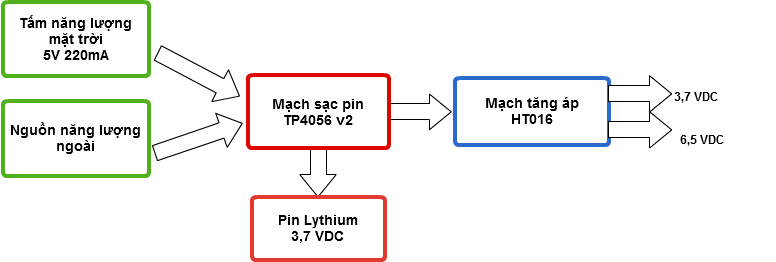
\includegraphics[width=6in]{khoinguon}
	\caption[Mô hình khối nguồn]{Mô hình khối nguồn}
	\label{fig:khoinguon}
\end{figure}

\begin{itemize}
	\item[•]Mạch tăng áp mini HT106 là module tăng áp cực kì nhỏ gọn, ngõ vào là cổng mircoUSB. Mạch có khả năng tăng đến 28v tối đa. Dưới đây là một số thông số kỹ thuật:\\
	-	Điện áp vào: 2-24V\\
	-	Điện áp ra: 5-28V\\
	-	Dòng tối đa: 2A đỉnh, dòng liên tục khoảng 1A.\\
	-	Công suất: 6W\\
	-	Hiệu suất: 93%
	\begin{figure}[H]
		\centering    
		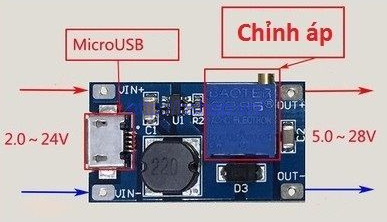
\includegraphics[width=3in]{ht06}
		\caption[Mạch tăng áp mini HT106]{Mạch tăng áp mini HT106}
		\label{fig:ht06}
	\end{figure}
	
	\item[•]Mạch sạc pin Lithium TP4056v2 sử dụng IC quản lý sạc TP4056 nhưng được nâng cấp để có thể ngắt khi pin yếu dưới 2.4V nhằm bảo vệ pin. Một số thông số kỹ thuật của mạch sạc pin Lithium TP4056v2\\
	-	Điện áp đầu vào: 5VDC mini USB\\
	-	Điện áp ngưỡng ra tự động ngắt: 4.2V +- 1%\\
	-	Dòng sạc tối đa: 1000mA\\
	-	Điện áp ngưỡng cần sạc là 2.5V\\
	-	Tích hợp tự động ngắt bảo vệ pin khi pin yếu dưới 2.4 V qua 2 chân OUT+ và OUT-
	\begin{figure}[H]
		\centering    
		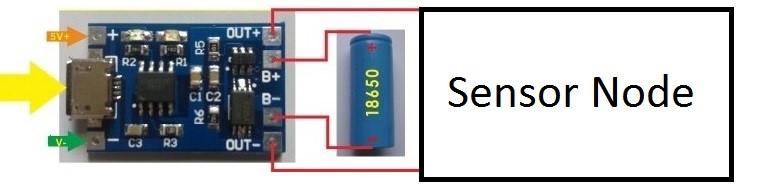
\includegraphics[width=5in]{tp4056}
		\caption[Mạch sạc pin Lithium TP4056v2]{Mạch sạc pin Lithium TP4056v2}
		\label{fig:tp4056}
	\end{figure}
	\item[•]Pin năng lượng mặt trời Poly 5.5V /220 mA\\
	-	Với kích thước: 100x80x2mm\\
	-	Nguồn đầu ra: 5.5V\\
	-	Dòng tối đa cung cấp được: 220mA\\
	\begin{figure}[H]
		\centering    
		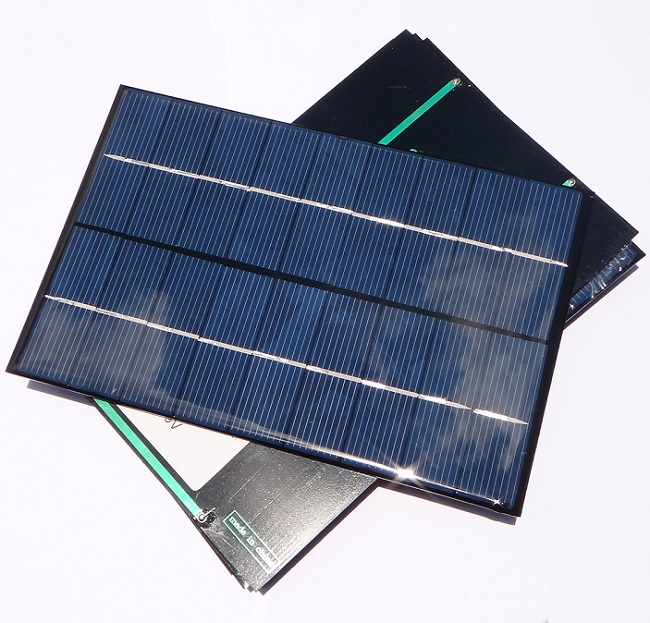
\includegraphics[width=0.6\textwidth]{solarpanel_real}
		\caption[Pin năng lượng mặt trời Poly 5.5V /220 mA]{Pin năng lượng mặt trời Poly 5.5V /220 mA}
		\label{fig:solarpanel_real}
	\end{figure}
	
	\item[•]Nguồn năng lượng ngoài: sử dụng trong một số trường hợp thời tiết mưa nhiều hoặc gió nhiều mà thiếu nguồn năng lượng mặt trời, chúng ta có thể tận dụng nguồn mưa và gió nhờ các tuapin phát năng lượng nhờ vào sức gió và mưa.
	\item[•] Nguồn đầu ra 3.7VDC dùng để cấp cho module Sim800L còn đối với nguồn 6.5VDC dùng để cung cấp cho mạch vi xử lý.
\end{itemize}

\newpage
\subsubsection*{Các thư viện đã sử dụng} 
\begin{lstlisting}[language=C]
#include "MQ135.h" //Thu vien cac ham toan hoc de xu ly so lieu MQ135
#include "MQ07.h" //Thu vien cac ham toan hoc de xu ly so lieu MQ07
#include "OneWire.h" // Thu vien cau hinh giao thuc I2C
#include "DallasTemperature.h" // Thu vien cho cam bien nhiet do
#include "SoftwareSerial.h" // Thu vien mo rong cac chan UART
#include "TimerOne.h" // Thu vien cau hinh timer
\end{lstlisting}



\subsubsection*{Kết quả hiện thực}
\begin{figure}[H]
	\centering    
	\includegraphics[width=5in]{prototype_2}
	\caption[Kết quả prototype đầu tiên]{Kết quả prototype đầu tiên}
	\label{fig:prototype_2}
\end{figure}

\begin{figure}[H]
	\centering    
	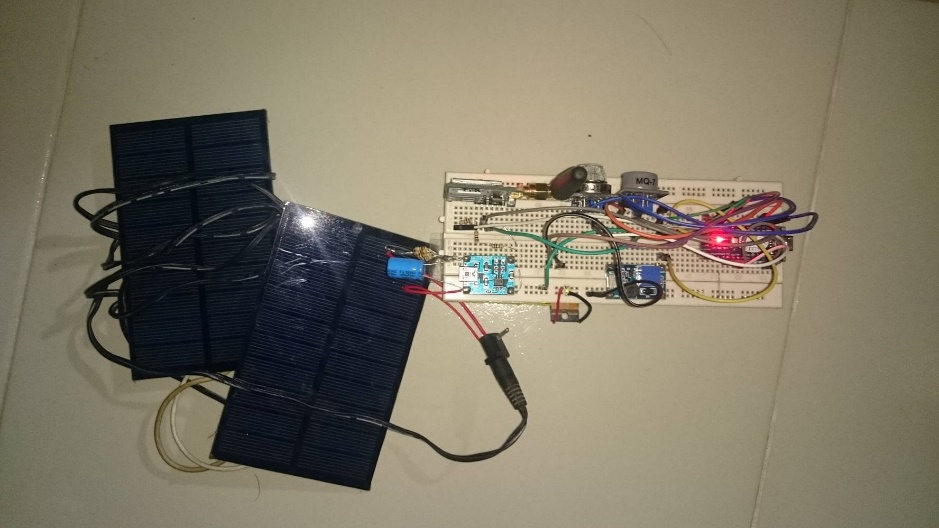
\includegraphics[width=5in]{prototype_3}
	\caption[Kết quả prototype đầu tiên 2]{Kết quả prototype đầu tiên 2}
	\label{fig:prototype_3}
\end{figure}



\subsubsection*{Nhận xét}
\begin{itemize}
	\item[•] Hoàn thành các chức năng có thể đọc được các dữ liệu từ cảm biến MQ135, MQ07, DS18B20, và GP2.
	\item[•] Xử lý được dữ liệu thông qua các thư viện do nhà sản xuất cảm biến cung cấp.
	\item[•] Gửi được dữ liệu lên máy chủ thông qua dịch vụ GPRS của Sim800L, hệ thống máy chủ của chúng tôi ban đầu chưa được hoàn thành nên nhờ đến công cụ phát triển IoT Thingspeak thì chúng tôi đã kiểm tra được, xem thêm tại: \url{https://thingspeak.com/channels/157120}
\end{itemize}



\newpage
\subsection{Hiện thực mô hình tổng thể node cảm biến}
\subsubsection*{Hiện thực board mạch vi xử lý}
Board mạch vi xử lý được thiết kế và hiện thực gọn nhất có thể và hỗ trợ các header nối các dây bus đến các cảm biến và module Sim800L. Chúng tôi đã thực hiện thiết kế board mạch vi xử lý như Hình \ref{fig:botrimcu}

\begin{figure}[H]
	\centering  
	\begin{subfigure}[b]{0.5\textwidth}
		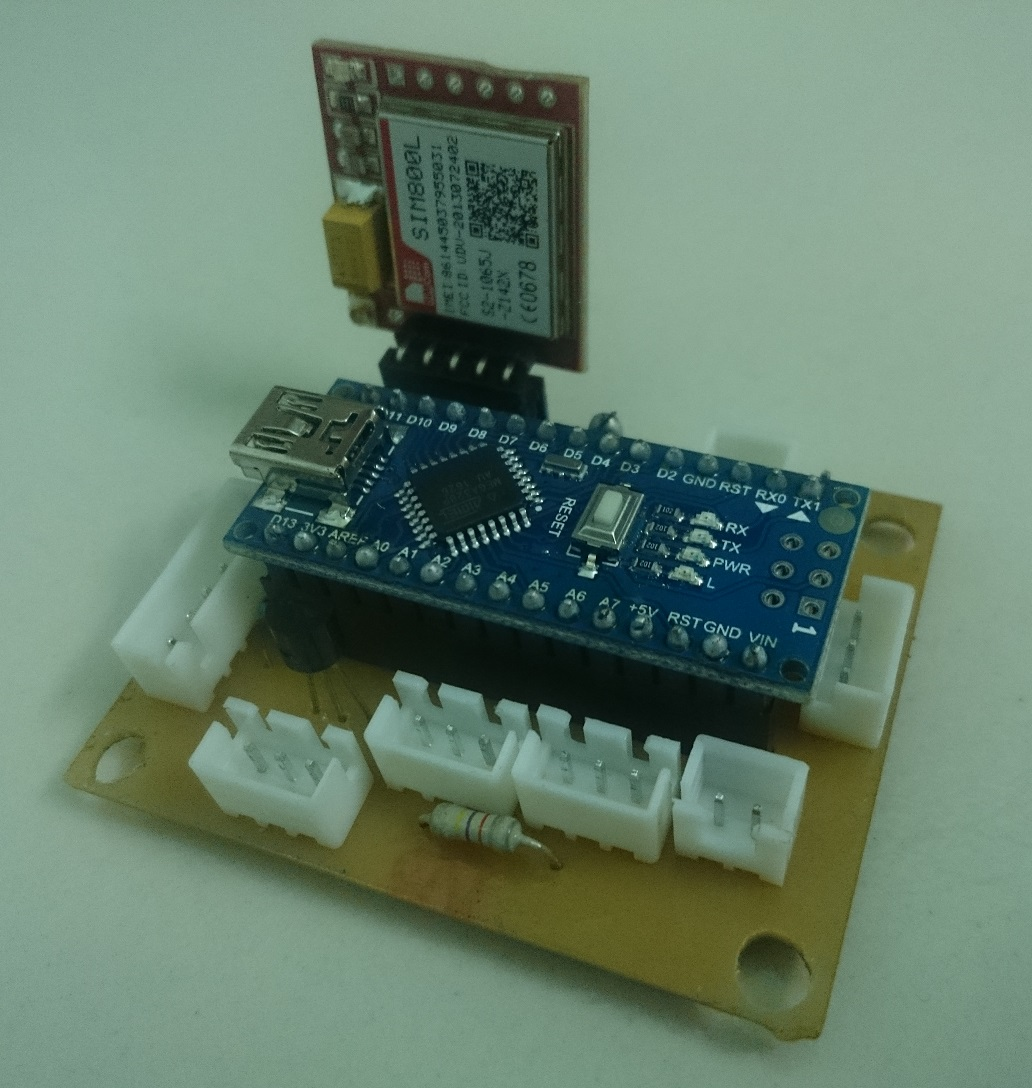
\includegraphics[width=3in]{mcu}
		\caption[Mô hình 1]{Mô hình 1}
		\label{fig:mcu}
	\end{subfigure}\hfill
	\begin{subfigure}[b]{0.5\textwidth}
		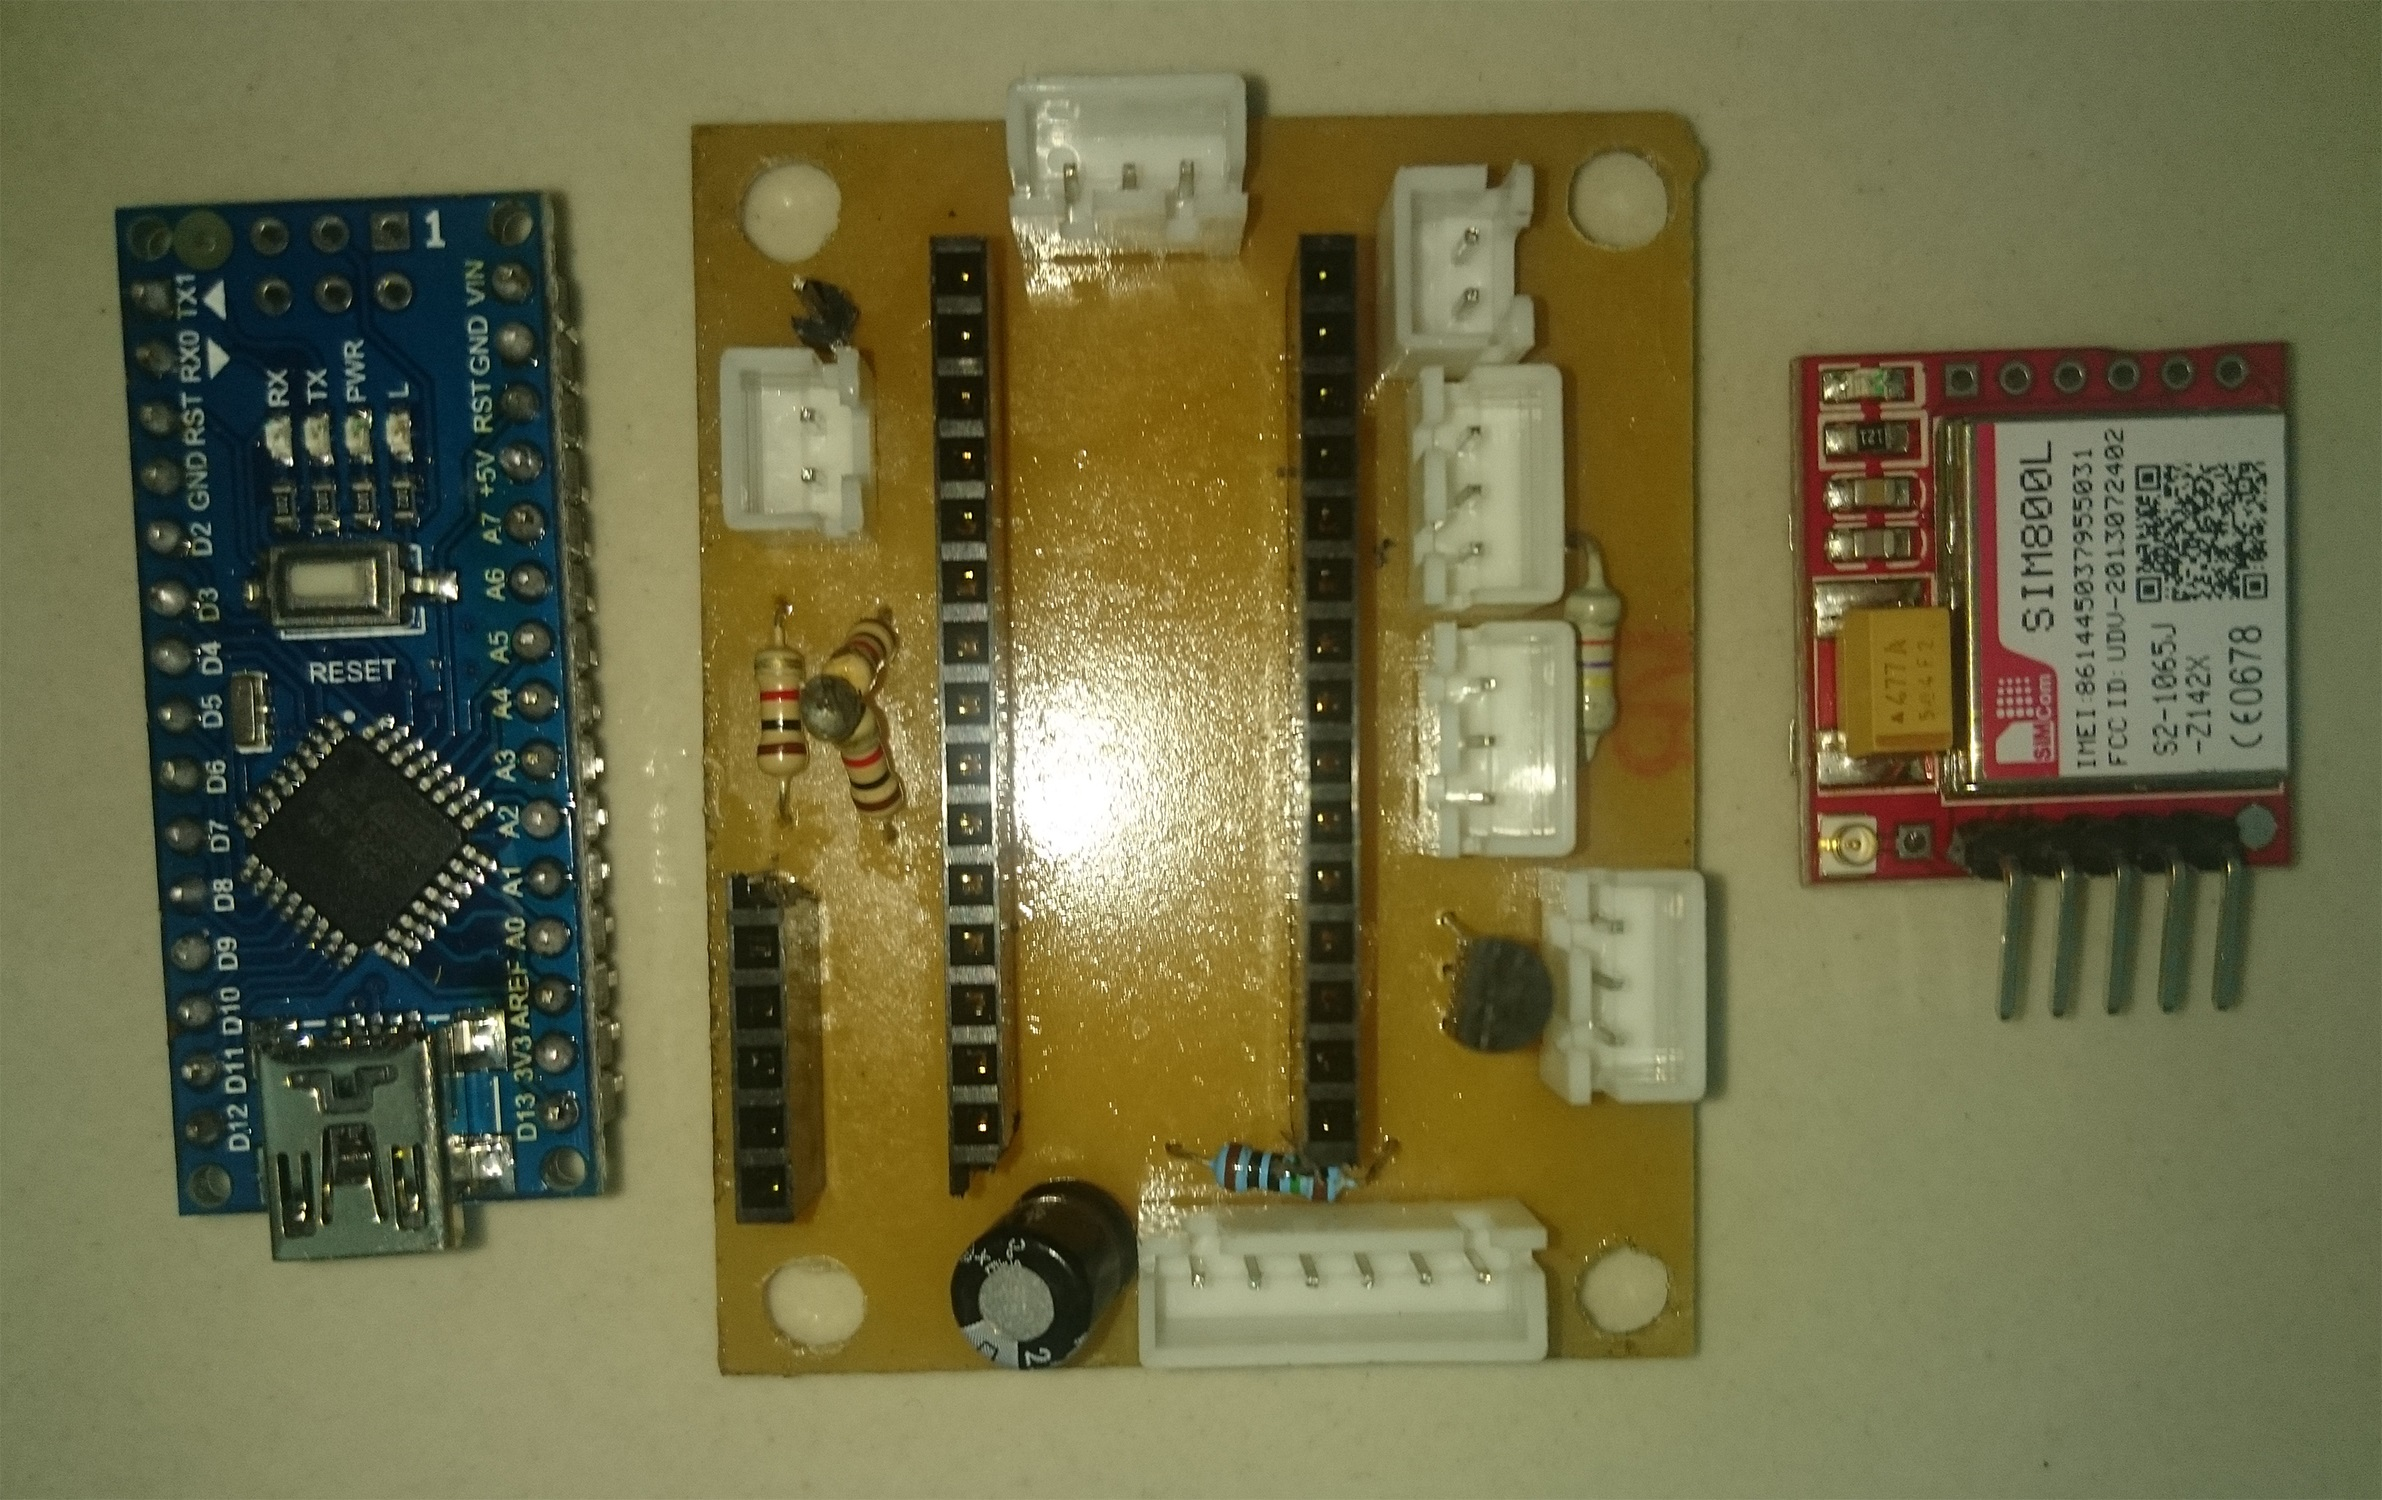
\includegraphics[width=3in]{mcu_2}
		\caption[Mô hình 2]{Mô hình 2}
		\label{fig:mcu_2}
	\end{subfigure}
	\caption{Bố trí board mạch vi xử lý}\label{fig:botrimcu}
\end{figure}

Một số khai báo được sử dụng như sau:
\begin{lstlisting}[numbers=left,firstnumber=1,language=C]
#define ONE_WIRE_BUS 4
#define MQ135_PIN A0
#define MQ7_PIN A1
#define RX_SIM_OUT 11
#define TX_SIM_OUT 10
#define DUST_OUT A2
#define DUST_PIN 2

// Gia tri % Pin thap se khong cho phep mach hoat dong
#define LOW_BATTERY 30 

// So lan gui lai du lieu len may chu neu khong thanh cong
#define TIMEFAIL_SENDSMS 5 

// Mo rong UART tren chan so 11 va 10
SoftwareSerial sim900(RX_SIM_OUT, TX_SIM_OUT);

int TIMEON = 3; //Thoi gian dot nong cam bien MQ135, MQ07

//Thoi gian ngat nguon cam bien MQ135, MQ07 ban ngay
int TIMEOFF_DAY = 13; 
//Thoi gian ngat nguon cam bien MQ135, MQ07 ban dem
int TIMEOFF_NIGHT = 28;

// Moc thoi gian xac dinh buoi sang va buoi toi
int time_s1 = 6;
int time_s2 = 19;

String apiKey = "7"; //Node ID
\end{lstlisting}
Lập trình cho vi xử lý Arduino Nano được mô hình hóa theo lưu đồ xử lý dưới Hình \ref{fig:node_status}:

\begin{figure}[H]
	\centering    
	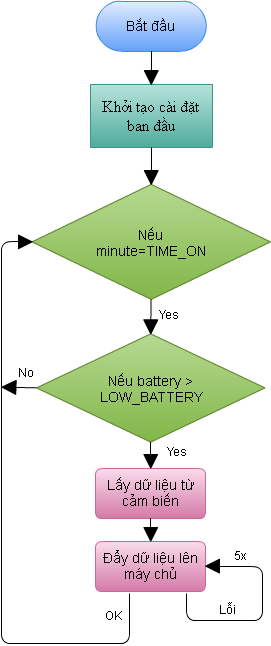
\includegraphics[width=2.5in]{node_status}
	\caption[Lưu đồ xử lý hàm main]{Lưu đồ xử lý hàm main}
	\label{fig:node_status}
\end{figure}

\begin{itemize}
	\item[•]Khởi tạo cài đặt ban đầu gồm các công việc: \\
	- Thiết lập chế độ hoạt động của các chân trên vi xử lý.\\
	- Thiết lập tốc độ truyền UART.\\
	- Thiết lập timer định thời.\\
	- Khởi động Module Sim800L.\\
	- Đồng bộ thời gian module Sim800L với máy chủ NTP.\\
	
	Việc Đồng bộ thời gian module Sim800L với máy chủ NTP được Sim800L hỗ trợ qua các tập lệnh sau:
	\begin{lstlisting}[numbers=left,firstnumber=1,language=C]
	void syncTime()
	{
	//  Network time sync
	sim900.println("AT+SAPBR=1,1");
	delay(2000);
	sim900.println("AT+CNTPCID=1");
	delay(2000);
	sim900.println("AT+CNTP=\"128.4.24.98\",28");
	delay(2000);
	sim900.println("AT+CNTP");
	delay(4000);  
	sim900.println("AT+SAPBR=0,1");
	delay(2000);
	Serial.println("Sync time - Done");
	updateTime();
	}
	\end{lstlisting}
	
	
	
	
	
	
	
\end{itemize}









\subsubsection*{Bố trí các linh kiện trong hộp cảm biến}
Việc bố trí các linh kiện trong hộp cảm biến nhầm giúp cho việc thu thập dữ liệu của các cảm biến được hiệu quả hơn và không bị ảnh hưởng bởi mưa. Nó cũng giúp cho việc phát triển trong tương lai nếu các cảm biến hoặc linh kiện bị hư thì dễ dàng thay thế hơn.

Đối với các cảm biến MQ135, MQ07 và cảm biến nhiệt DS18B20 thì được bố trí đặt ở lớp dưới của chiếc hộp như Hình \ref{fig:botri}

\begin{figure}[H]
	\centering  
	\begin{subfigure}[b]{0.5\textwidth}
		
\includegraphics[width=2.5in]{house_sensor}
		\caption[Mô hình]{Mô hình}
		\label{fig:house_sensor}
	\end{subfigure}\hfill
	\begin{subfigure}[b]{0.5\textwidth}
		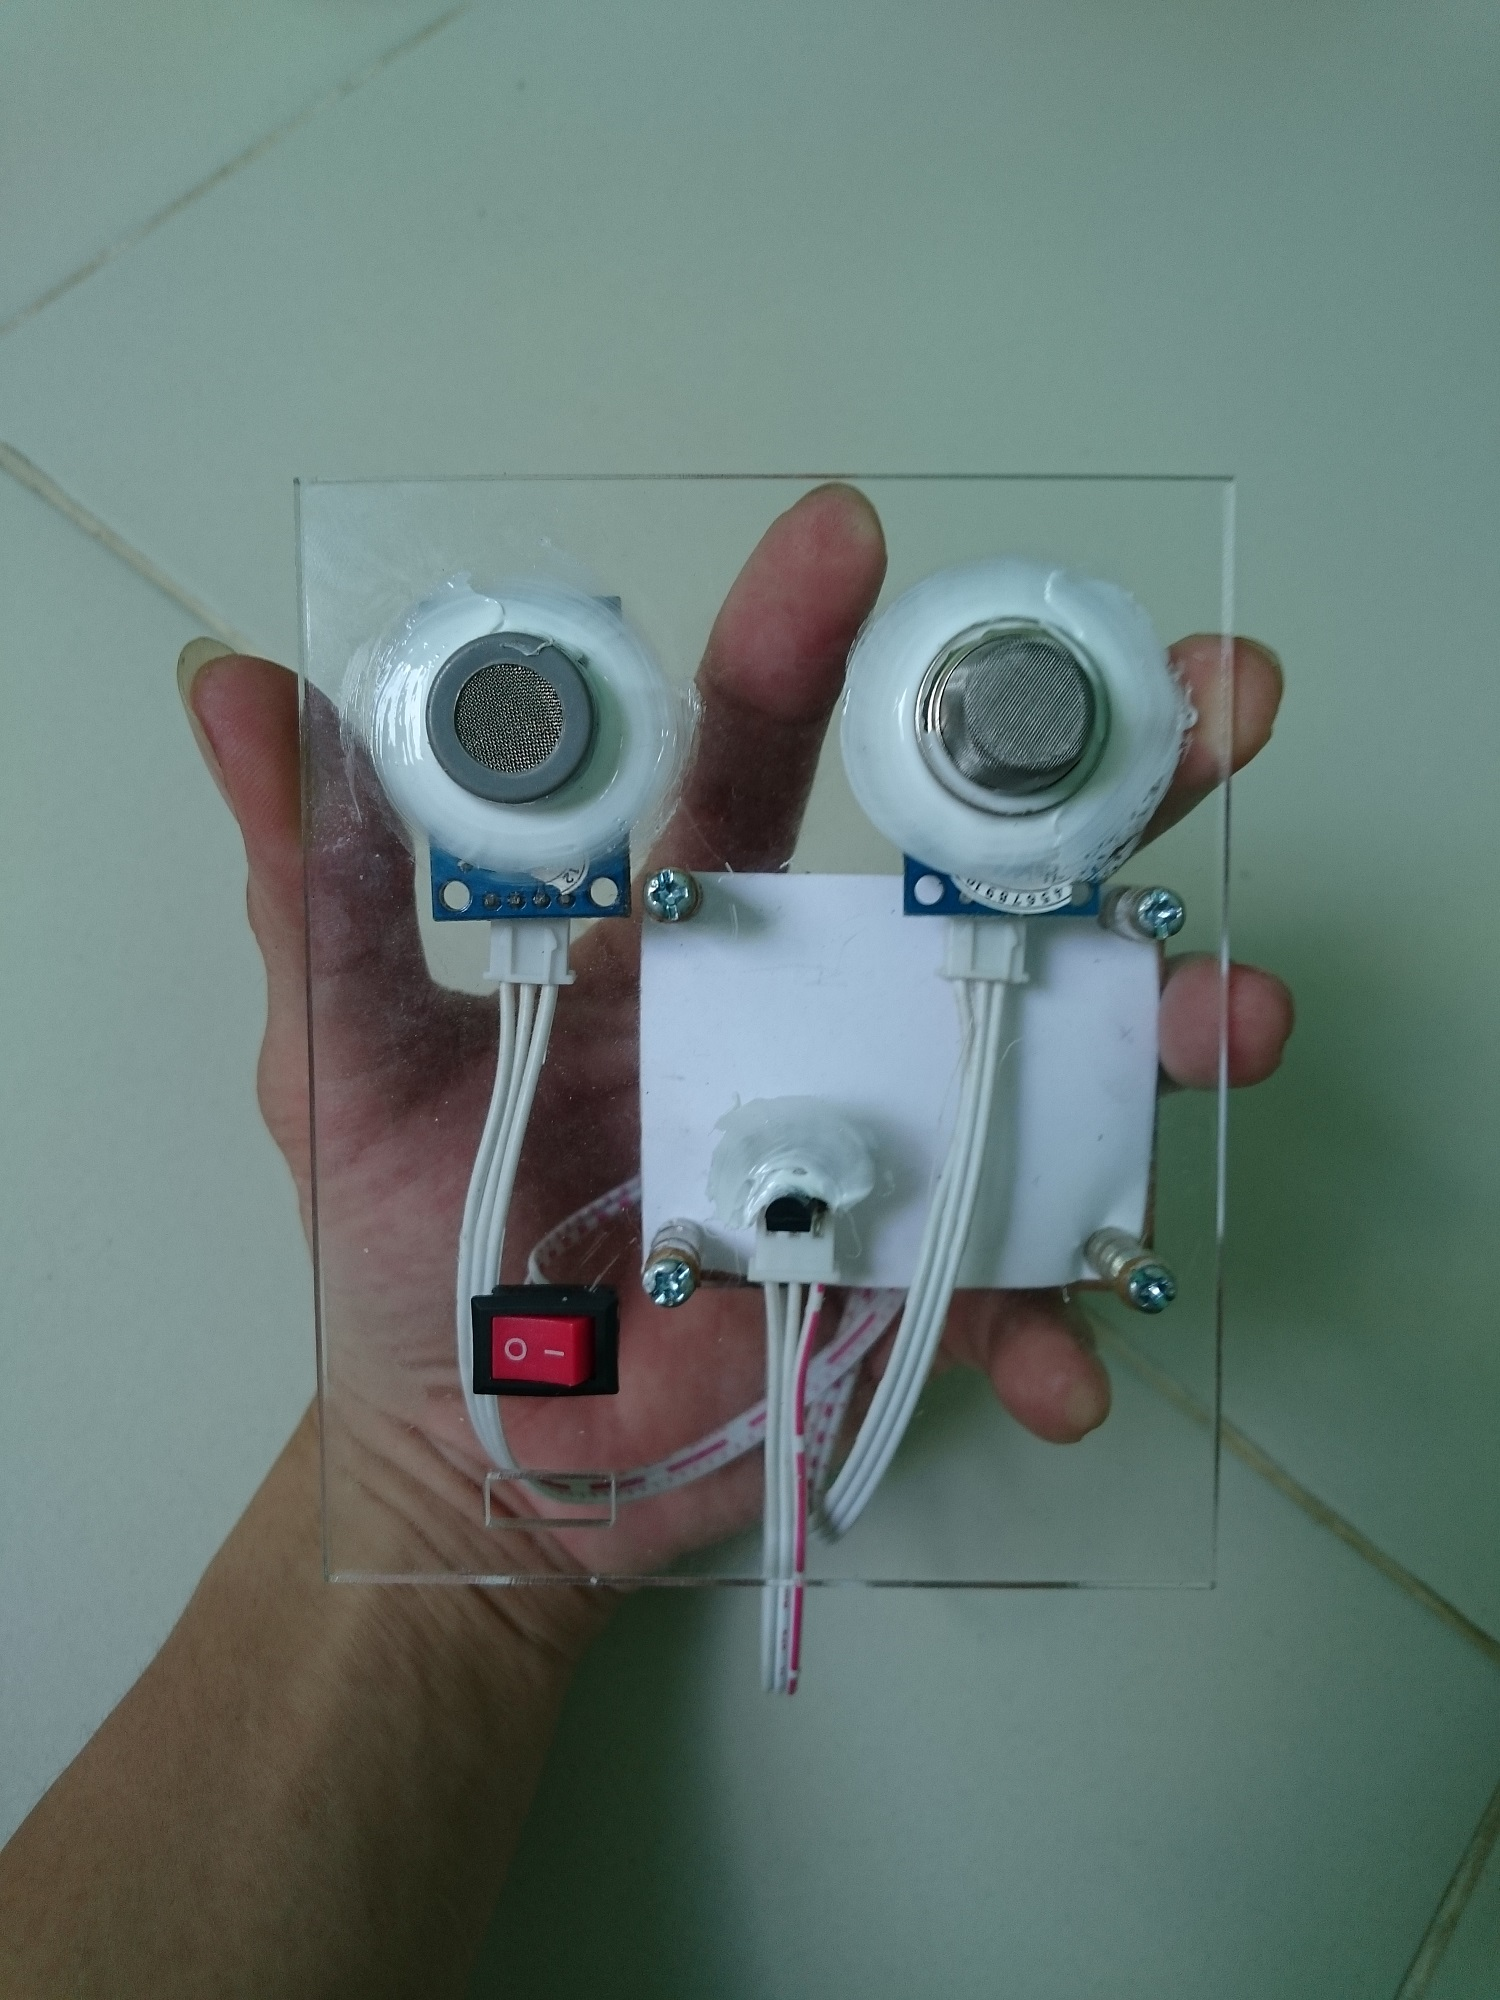
\includegraphics[width=2.5in]{house_sensor_2}
		\caption[Thực tế]{Thực tế}
		\label{fig:house_sensor_2}
	\end{subfigure}
	\caption{Bố trí các cảm biến}\label{fig:botri}
\end{figure}
Đối với các cảm biến bụi GP2 chúng tôi đề xuất vị trí được đặt như Hình \ref{fig:house_dust} sau:
\begin{figure}[H]
	\centering    
	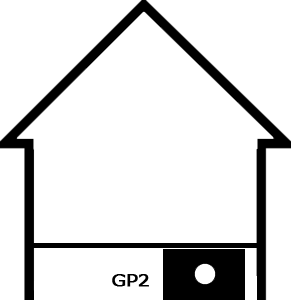
\includegraphics[width=2.5in]{house_dust}
	\caption[Mô hình đặt cảm biến GP2]{Mô hình đặt cảm biến GP2}
	\label{fig:house_dust}
\end{figure}
Còn các board mạch vi xử lý, module Sim800L và pin được đặc vị trí bên trong chiếc hộp như Hình \ref{fig:botrikhac} sau:
\begin{figure}[H]
	\centering  
	\begin{subfigure}[b]{0.5\textwidth}
		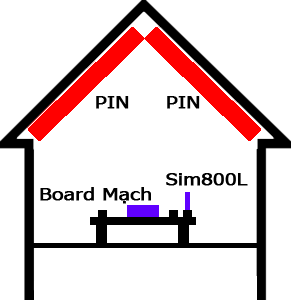
\includegraphics[width=2.5in]{house_board_kogps}
		\caption[Mô hình]{Mô hình}
		\label{fig:house_board_kogps}
	\end{subfigure}\hfill
	\begin{subfigure}[b]{0.5\textwidth}
		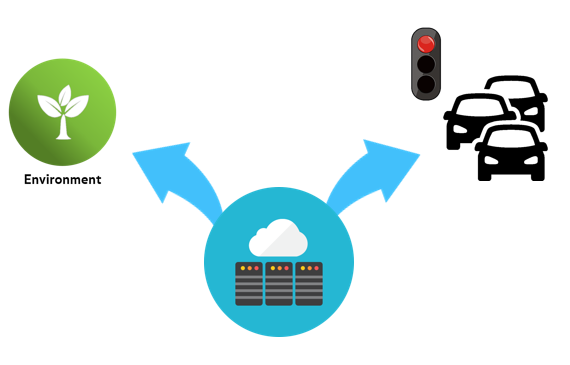
\includegraphics[width=2.5in]{pic1}
		\caption[Thực tế]{Thực tế}
		\label{fig:pic1}
	\end{subfigure}
	\caption{Bố trí các cảm biến khác}\label{fig:botrikhac}
\end{figure}
\subsection{Mức độ tiêu hao năng lượng}
Để biết được mức tiêu hao năng lượng của mạch hoạt động như thế nào thì chúng tôi đã bắt đầu tính toán từ những thông số tiêu thụ chuẩn của các linh kiện được sử dụng trong node cảm biến. Nhầm nắm bắt được và đưa ra dung lượng pin cần thiết cho các node cảm biến chạy mà không phụ thuộc vào mạng lưới điện.

Chú ý: các thông số tính toán dưới lấy từ thông số chuẩn của nhà sản xuất kèm với một số thông số chuẩn của chúng tôi như sau:
\begin{itemize}
	\item[•] Thời gian cho việc đốt nóng cảm biến MQ135 và MQ07 trước khi lấy dữ liệu: 3 phút
	\item[•] Ban ngày từ 7AM-8PM: cứ mỗi 15 phút gửi dữ liệu lên máy chủ.
	\item[•] Ban đêm từ 8PM-7AM: cứ mỗi 30 phút gửi dữ liệu lên máy chủ.
\end{itemize}

\textbf{Mức tiêu hao năng lượng vào 1 buổi sáng 7AM-8PM:}
\begin{table}[H]
	\centering
	\caption{Bảng tiêu thụ năng lượng buổi sáng}
	\label{table:buoisang}
	\begin{tabular}{|l|l|r|r|r|r|}
		\hline
		\textbf{STT}  & \textbf{Module}                                                       & \multicolumn{1}{c|}{\textbf{\begin{tabular}[c]{@{}c@{}}Dòng tiêu \\ thụ (mA)\end{tabular}}} & \multicolumn{1}{c|}{\textbf{\begin{tabular}[c]{@{}c@{}}Giờ hoạt \\ động (h)\end{tabular}}} & \multicolumn{1}{c|}{\textbf{\begin{tabular}[c]{@{}c@{}}Tổng dòng \\ tiêu thụ(mA)\end{tabular}}} & \multicolumn{1}{c|}{\textbf{\begin{tabular}[c]{@{}c@{}}Công suất\\ (mW)\end{tabular}}} \\ \hline
		1             & Cảm biến bụi                                                          & 20                                                                                          & 13                                                                                         & 260                                                                                             & 858                                                                                    \\ \hline
		2             & Cảm biến MQ07                                                         & 250                                                                                         & 2.6                                                                                        & 650                                                                                             & 3250                                                                                   \\ \hline
		3             & Cảm biến MQ135                                                        & 300                                                                                         & 2.6                                                                                        & 780                                                                                             & 3900                                                                                   \\ \hline
		4             & \begin{tabular}[c]{@{}l@{}}Cảm biến nhiệt độ\\ 18BS20\end{tabular}    & 1.5                                                                                         & 13                                                                                         & 19.5                                                                                            & 97.5                                                                                   \\ \hline
		5             & \begin{tabular}[c]{@{}l@{}}Module Sim800L \\ (idea mode)\end{tabular} & 10                                                                                          & 12.35                                                                                      & 123.5                                                                                           & 456.95                                                                                 \\ \hline
		6             & \begin{tabular}[c]{@{}l@{}}Module Sim800L\\ (Hoạt động)\end{tabular}  & 500                                                                                         & 0.65                                                                                       & 325                                                                                             & 1202.5                                                                                 \\ \hline
		7             & Arduino nano                                                          & 10                                                                                          & 13                                                                                         & 130                                                                                             & 780                                                                                    \\ \hline
		\textbf{Tổng} & \textbf{}                                                             & \textbf{1091.5}                                                                             & \textbf{}                                                                                  & \textbf{2288}                                                                                   & \textbf{10544.95}                                                                      \\ \hline
	\end{tabular}
\end{table}

\textbf{Mức tiêu hao năng lượng vào 1 buổi tối 8PM-7AM:}
\begin{table}[H]
	\centering
	\caption{Bảng tiêu thụ năng lượng buổi tối}
	\label{table:buoitoi}
	\begin{tabular}{|l|l|r|r|r|r|}
		\hline
		\textbf{STT}  & \textbf{Module}                                                       & \multicolumn{1}{c|}{\textbf{\begin{tabular}[c]{@{}c@{}}Dòng tiêu \\ thụ (mA)\end{tabular}}} & \multicolumn{1}{c|}{\textbf{\begin{tabular}[c]{@{}c@{}}Giờ hoạt \\ động (h)\end{tabular}}} & \multicolumn{1}{c|}{\textbf{\begin{tabular}[c]{@{}c@{}}Tổng dòng \\ tiêu thụ(mA)\end{tabular}}} & \multicolumn{1}{c|}{\textbf{\begin{tabular}[c]{@{}c@{}}Công suất\\ (mW)\end{tabular}}} \\ \hline
		1             & Cảm biến bụi                                                          & 20                                                                                          & 11                                                                                         & 220                                                                                             & 726                                                                                    \\ \hline
		2             & Cảm biến MQ07                                                         & 250                                                                                         & 2.2                                                                                        & 550                                                                                             & 2750                                                                                   \\ \hline
		3             & Cảm biến MQ135                                                        & 300                                                                                         & 2.2                                                                                        & 660                                                                                             & 3300                                                                                   \\ \hline
		4             & \begin{tabular}[c]{@{}l@{}}Cảm biến nhiệt độ\\ 18BS20\end{tabular}    & 1.5                                                                                         & 11                                                                                         & 16.5                                                                                            & 82.5                                                                                   \\ \hline
		5             & \begin{tabular}[c]{@{}l@{}}Module Sim800L \\ (idea mode)\end{tabular} & 10                                                                                          & 10.45                                                                                      & 104.5                                                                                           & 386.65                                                                                 \\ \hline
		6             & \begin{tabular}[c]{@{}l@{}}Module Sim800L\\ (Hoạt động)\end{tabular}  & 500                                                                                         & 0.55                                                                                       & 275                                                                                             & 1017.5                                                                                 \\ \hline
		7             & Arduino nano                                                          & 10                                                                                          & 11                                                                                         & 110                                                                                             & 660                                                                                    \\ \hline
		\textbf{Tổng} & \textbf{}                                                             & \textbf{1091.5}                                                                             & \textbf{}                                                                                  & \textbf{1936}                                                                                   & \textbf{8922.65}                                                                       \\ \hline
	\end{tabular}
\end{table}

\section{Hệ thống Server lưu trữ dữ liệu và cung cấp API}

\subsection{Cấu trúc tổ chức tập tin}
\subsubsection*{Các thư mục và chức năng}
Chúng ta có những thư mục được làm việc trực tiếp:

• \textbf{libs}: chứa các hàm function hỗ trợ về xác thực và log.

• \textbf{models}: thư mục này bao gồm các mô hình quản lý cơ sở dữ liệu.

• \textbf{routes}: điều khiển và điều hướng theo các url.

• \textbf{log}: chứa các file ghi lại log trong quá trình hoạt động.

• \textbf{views}: là bộ mặt của web server, giúp người dùng có thể tương tác được với server qua web browser, bao gồm các file giao diện như html, ejs...   


\subsubsection*{Các file khởi tạo và cấu hình Server}

\textbf{Các file khởi tạo này bao gồm:}

• \textbf{emap.js}: file có chức năng đọc file cấu hình và khởi tạo kết nối server.
\begin{lstlisting}[caption=emap.js]
...
server.on('listening', onListening); // open for listening
function onListening() {
var addr = server.address();
var bind = typeof addr === 'string' ?
'pipe' + addr :
'port' + addr.port;
debug('Listening on ' + bind);
console.log('Listening on ' + bind);
};
...
\end{lstlisting}

• \textbf{app.js}: là file điều khiển và thiết lập các chức năng, khai báo các modules chính được sử dụng. Bên cạnh đó, còn có chức năng gán điều hướng tới các file trong thư mục route
\begin{lstlisting}[caption=app.js]
...
// initial server
app.use(passport.initialize());
app.use(passport.session());
app.set('views', path.join(\_\_dirname, 'views'));
app.engine('ejs', engine);
...
// control route
app.use(logger('dev'));
app.use('/log', express.static(path.join(__dirname, 'log')));
app.use(express.static(path.join(__dirname, 'public')));
app.use('/log', serveIndex('./log'));
app.use('/', routes);
app.use('/user', user);
app.use('/node', node);
app.use('/auth', auth);
...
\end{lstlisting}

\textbf{Các file cấu hình này bao gồm:}

• \textbf{package.json}: khai báo các thông tin cơ bản về project và các modules được sử dụng.
\begin{Verbatim}[xleftmargin=2em]
{
"name": "emap-server",
"version": "1.0.0",
"description": "This is serverside part of IoT project",
"main": "emap.js",
"author": "Cuong, Tung and Ny",
"license": "ISC",
"homepage": "www.codingyourfuture.com",
"dependencies": {// dependancies modules
"angular-chart.js": "^1.0.3",
"asyncawait": "^1.0.6",
"babel": "^6.5.2",
"ejs": "^2.5.2",
...
"rethinkdb": "^2.3.3",
"serve-index": "^1.8.0",
"socket.io": "^1.5.0",
}
}
\end{Verbatim}
• \textbf{config.json}: khai báo các thông số cấu hình được sử dụng. Tại đây ta cấu hình thông số kết nối tới RethinkDB và port ứng dụng server nodejs.
\begin{Verbatim}[xleftmargin=2em]
{
"app":{
"port": "8888"
},
"rethinkdb":{
"host": "localhost",
"port" : "28015",
"db": "emap",
"address":"localhost:28015",
"tableList":["nodeData","nodeList","user"]
}
}

\end{Verbatim}


%% Thiết kế API



\subsection{Xây dựng Database}
% TODO: node cảm biến hay sensor node?
Hệ quản lý cơ sở dữ liệu được sử dụng tại hệ thống là RethinkDB như mô hình thiết kế hệ thống tại mục \ref{sec:struc} . Cơ sở dữ liệu được chia làm 3 bảng: nodeList, nodeData và user được miêu tả tại các hình \ref{fig: dbnode} và\ref{fig: dbuser}

Các dữ liệu về node được chia làm hai bảng:

• nodeList: chứa các thông tin về các sensor node, trong đó data\_id đóng vai trò tương tự như foreign key của bảng nodeData để có thể truy xuất dữ liệu.

• nodeData: tập trung những dữ liệu thu thập được từ các sensor node theo thời gian thực. 
\begin{figure}[H]
	\centering    
	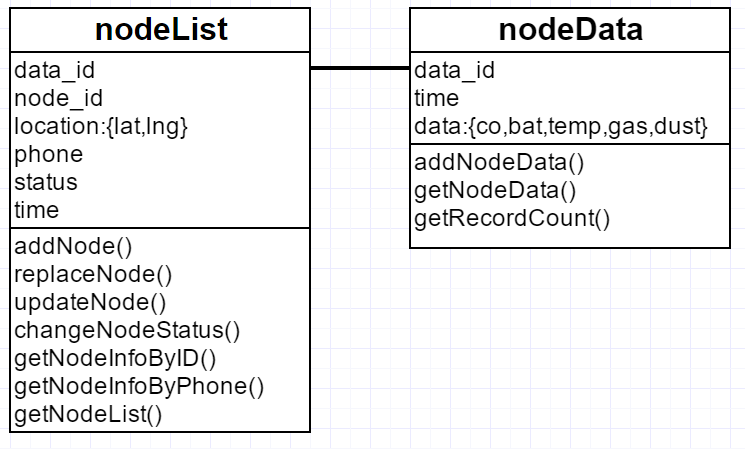
\includegraphics[width=1.0\textwidth]{dbnode}
	\caption[Mô hình cấu trúc dữ liệu của Sensor Node]{Mô hình cấu trúc dữ liệu của Sensor Node}
	\label{fig: dbnode}
\end{figure}
Về phía user, chỉ có một bảng quản lý người dùng bao gồm các thông tin cơ bản để xác thực và quyền thay đổi chỉnh sửa dữ liệu sensor node.
\begin{figure}[H]
	\centering    
	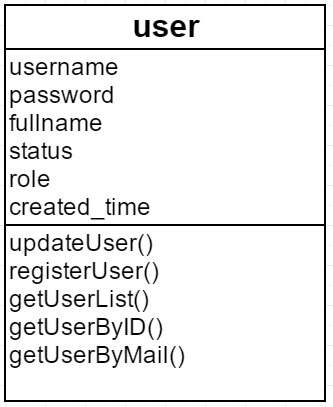
\includegraphics[width=0.45\textwidth]{dbuser}
	\caption[Mô hình cấu trúc dữ liệu của User]{Mô hình cấu trúc dữ liệu của User}
	\label{fig: dbuser}
\end{figure}

Vì mục hệ thống phát triển dừng ở mức xây dựng và thiết kế hệ thống thu thập và truy vấn dữ liệu từ các sensor node nên chưa có bảng phân quyền sở hữu giữa người dùng và sensor node.
\subsection{Hiện thực API}
Dựa trên mô hình thiết kế API tại \ref{sec: api}, API được hiện thực và phát triển.


\subsubsection*{API đăng ký và xác thực người dùng}

Các API này được xây dựng để quản lý và phân quyền người dùng, cho phép sử dụng các API về quản lý thông tin của các sensor node.

\textbf{Đăng nhập:}

Hệ thống sử dụng module Passport chạy trên nền Nodejs, có chức năng dễ dàng thiết lập xác thực người dùng. Module này có thể liên kết với các tài khoản phổ biến như Facebook, Google, Twitter... để hỗ trợ phương thức đăng nhập tiện lợi nhất cho người dùng. Tuy nhiên hệ thống chỉ sử dụng phương thức đăng nhập và quản lý người dùng ở mức local vì là phương thức phù hợp với đề tài.

Chi tiết API đăng nhập:
\begin{Verbatim}[xleftmargin=2em]
POST: /auth/login
data: {username,password}
======================
RESPOND:
case Success:
{
code: 1,
username,
message: 'Login successful'
}
case Failure	
{
code: 0,
message: "Invalid username or password"
}
======================
\end{Verbatim}

\textbf{Lưu thông tin người dùng bằng session:}

Sau khi đăng nhập, một session, còn gọi là phiên làm việc, sẽ được hình thành và lưu trữ trong thời gian nhất định. Session cho phép người dùng có thể vào các trang quản lý với quyền hạn cho phép mà không yêu cầu đăng nhập lại, cũng như được phép sử dụng các API quản lý sensor node.

Session sẽ tự động xóa sau một thời gian quy định, cụ thể ở hệ thống này là 10 ngày kể từ lần đăng nhập gần nhất. Người dùng có thể xóa thủ công bằng cách đăng xuất qua phương thức:
\begin{Verbatim}[xleftmargin=2em]
GET: /auth/logout
======================
RESPOND:
case Success:
{
code: 1,
message: "User has logged out"
}
case Failure:	
{
code: 0,
message: "User has not logged in yet"
}	
\end{Verbatim}

Quá trình đăng nhập và tạo session được mô tả như hình \ref{fig: apilogin}

\begin{figure}[H]
	\centering    
	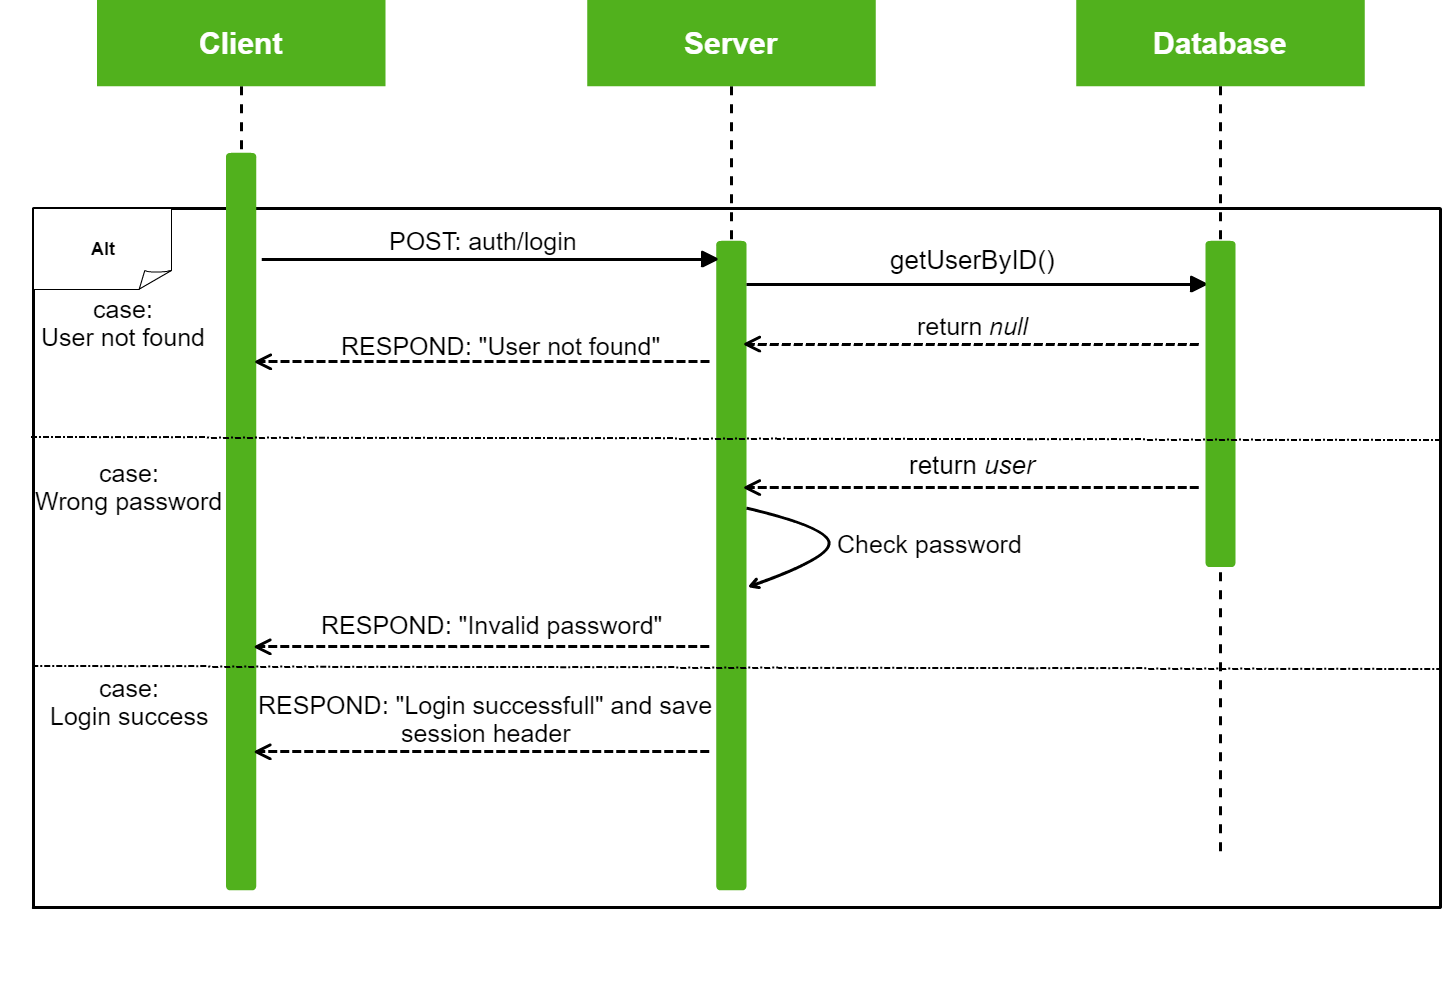
\includegraphics[width=1\textwidth]{apilogin}
	\caption[Quá trình đăng nhập và tạo session]{Quá trình đăng nhập và tạo session}
	\label{fig: apilogin}
\end{figure}


\textbf{Đăng ký:}

\begin{Verbatim}[xleftmargin=2em]
POST: /user/register
data:{username, password, name, mail}
======================	
RESPOND:
{
code: -1,
message: "Username existed"
}
{
code: -2,
message: "Mail is used",
}
{
code: 1,
message: "Account created successful"
}
======================	
\end{Verbatim}
\subsubsection*{API cung cấp và quản lý sensor node}
Các API được miêu tả tại bảng \ref{table: apilist}, các request và respond được miêu tả chi tiết:

• API thiết lập và cấu hình các sensor node: initnew, updatenode và replace node yêu cầu phải có đăng nhập từ API xác thực người dùng để giữ session và sau đó mới có thể sử dụng. Các API này có cấu trúc tương tự nhau và được mô tả:
\begin{Verbatim}[xleftmargin=2em]
POST: /node/initnew
data: {node_id,lat,lng,phone,status}
======================
RESPOND:
case Success:
{
code: 1,
message: 'Add node successful'
}
case Duplicated:
{
code: 0,
message: 'Node duplicated'
}
case Failure:
{
code: 0,
message: 'Add node failure'
}
case Not authenticated:
{
code: -1,
message: 'You are not authenticated'
}
======================	

\end{Verbatim}
Quá trình đăng nhập và tạo session được mô tả như hình \ref{fig: apipost}

\begin{figure}[H]
	\centering    
	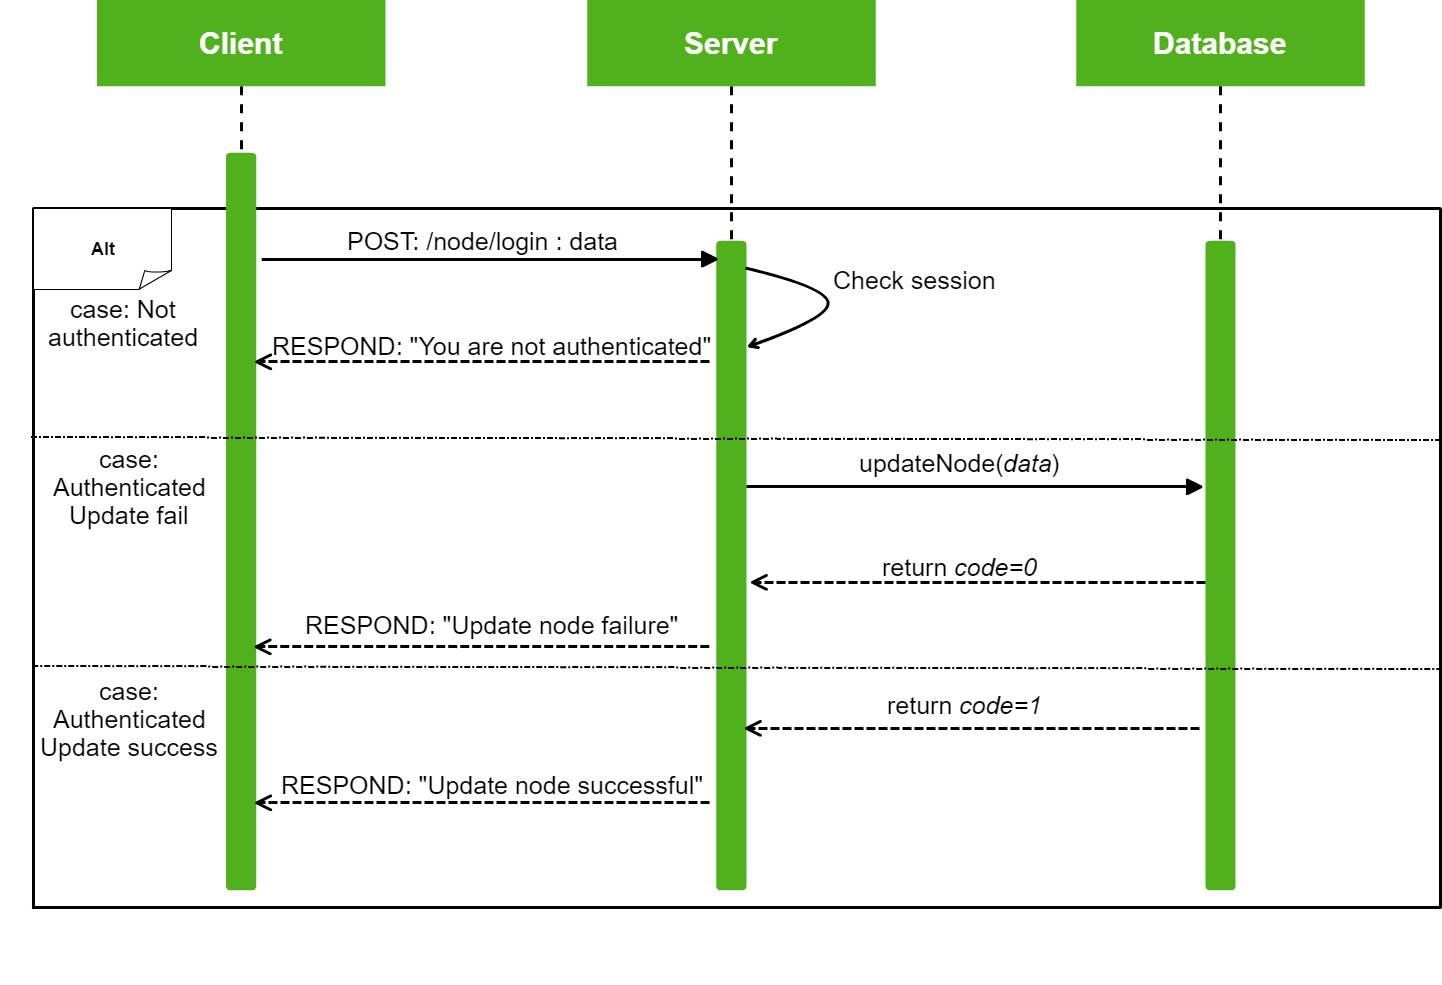
\includegraphics[width=1\textwidth]{apipost}
	\caption[Quá trình kiểm tra session của API POST]{Quá trình kiểm tra session của API POST}
	\label{fig: apipost}
\end{figure}

• API get thông tin và dữ liệu các sensor node: sử dụng phương thức GET để truy xuất dữ liệu về thông tin sensor node và dữ liệu các cảm biến. Hệ thống được thiết kế mang tính mở và chia sẻ nên không yêu cầu đăng nhập để truy xuất dữ liệu. Các thông tin đặc tả chi tiết API:
\begin{Verbatim}[xleftmargin=2em]
GET:	/node/getinfo?*query
Ex: 	/node/getinfo?id=1&status=0
/node/getinfo?list=1&status=1
Query:
+ id=*node ID* để get node bằng ID
+ phone: *node phonenumber* để get node bằng phone number
+ list=1 để get list các node
+ status=1 để get node đang ở trạng thái active,= 0 để node ở tất cả 
trạng thái, cũng như lịch sử thay đổi node
======================
RESPOND:
data:
- single node:{node_id,location:{lat,lng},phone,,time,data_id,status}
- list: array of {node_id,location:{lat,lng},phone,time,data_id,status}
======================
\end{Verbatim}

• API push dữ liệu từ sensor node: cũng tương tự như API get dữ liệu, API push dữ liệu sử dụng method GET thay cho POST để hỗ trợ dễ dàng trong việc thiết lập các thiết bị IoT đóng góp dữ liệu. Lượng dữ liệu của các sensor node không quá lớn, chỉ bao gồm những trường sensor ID và node ID nên có thể tích hợp vào thanh header của request.

\begin{Verbatim}[xleftmargin=2em]
GET: 	/node/pushdata?*query
Ex: 	/node/pushdata?node_id=1&s1=22&s2=33&s3=44&s4=55&s5=66
Query:
+ node_id: node ID
+ s1,s2,s3,s4,s5: value of each sensor
======================
RESPOND:
case Success:
{
code: 1,
message: 'Add node data successful'
}
case Failure:	
{
code: 0,
message: 'Add node data failure'
}
======================
\end{Verbatim}

\subsubsection*{Cung cấp API log}

Để hỗ trợ bên nhà phát triển thứ ba ứng dụng API tốt hơn, hệ thống có cung cấp các thông tin hoạt động của server, các request và respond cũng như các dữ liệu được truy vấn. Khi truy cập vào đường dẫn /log/, chúng ta sẽ có những file log tương ứng với các ngày như hình \ref{fig: log} :

\begin{figure}[H]
	\centering    
	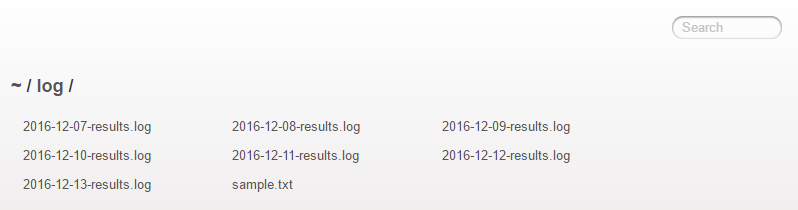
\includegraphics[width=1.0\textwidth]{log}
	\caption[Hiển thị các file log]{Hiển thị các file log}
	\label{fig: log}
\end{figure}

Ví dụ cụ thể của một đoạn log:
\begin{lstlisting}
{"level":"info","message":"IP:123.151.42.61 GET /route","timestamp":"10:48:56"}
{"level":"info","message":"IP:14.161.14.94 GET /statis route","timestamp":"10:49:22"}
{"level":"info","message":"IP:14.161.14.94 GET /graph route","timestamp":"10:49:27"}
{"level":"info","message":"IP:14.161.14.94 GET /node/getinfo: get list node info - number of nodes 12","timestamp":"10:49:27"}
{"level":"info","message":"IP:14.161.14.94 GET /node/getinfo: get node info by id:9","timestamp":"10:49:29",{"data_id":"106c59fe-753d-4a76-8418-88fd0df68d0c","id":"87b7f859-8c1e-4608-9645-5105ebb38e9b", "location":{"lat":10.91085286140159,"lng":106.99790954589844}, "node_id":"9","phone":"0123456899","status":1,"time":"2016-12-06T02:08:57.943Z"}}
{"level":"info","message":"IP:14.161.14.94 GET /node/getdata: Node data ID 9 number of records:  120","timestamp":"10:49:29"}
\end{lstlisting}

Các thông tin được thể hiện trong file log đủ thông tin để cho phép nhà phát triển theo dõi và áp dụng trong việc hiện thực sản phẩm.
\subsection{Xây dựng Web Server}

\subsection{Hiện thực giao diện}

Sử dụng framework express của Nodejs và HTML để xây dựng frontend

\subsubsection*{Giao diện chính của Web Server}
Phần này chứa các nút menu chức năng cùng với google map để theo dõi vị trí hoạt động của các cảm biến.
\begin{center}
	\begin{figure}[H]
		\centering    
		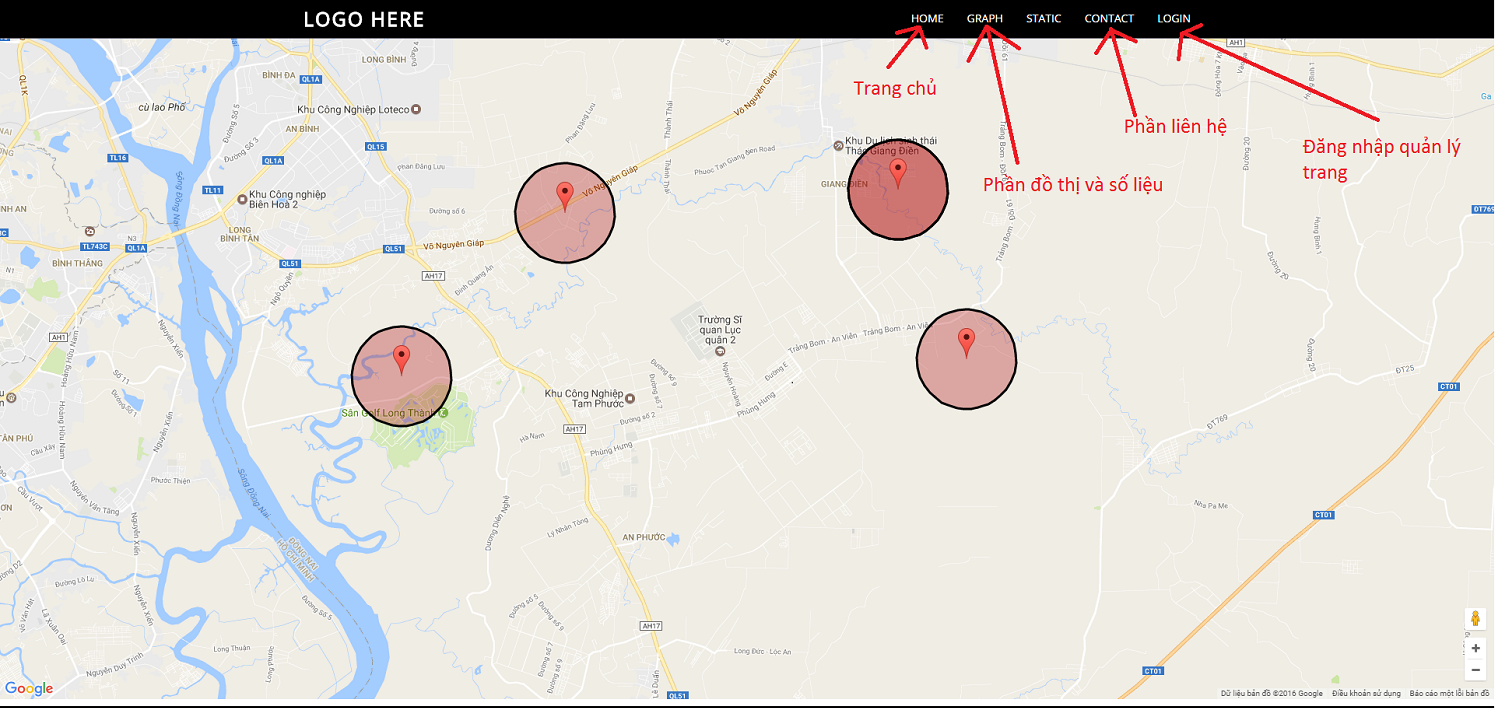
\includegraphics[width=1\textwidth]{webserver}
		\caption[Giao diện chính của Web Server]{Giao diện chính của Web Server}
		\label{fig:webserver}
	\end{figure}
\end{center}

\subsubsection*{Giao diện đồ thị dữ liệu}
Là nơi hiện thị biểu đồ của các thông số cũng như thông tin tương ứng của các cảm biến.
\begin{center}
	\begin{figure}[H]
		\centering    
		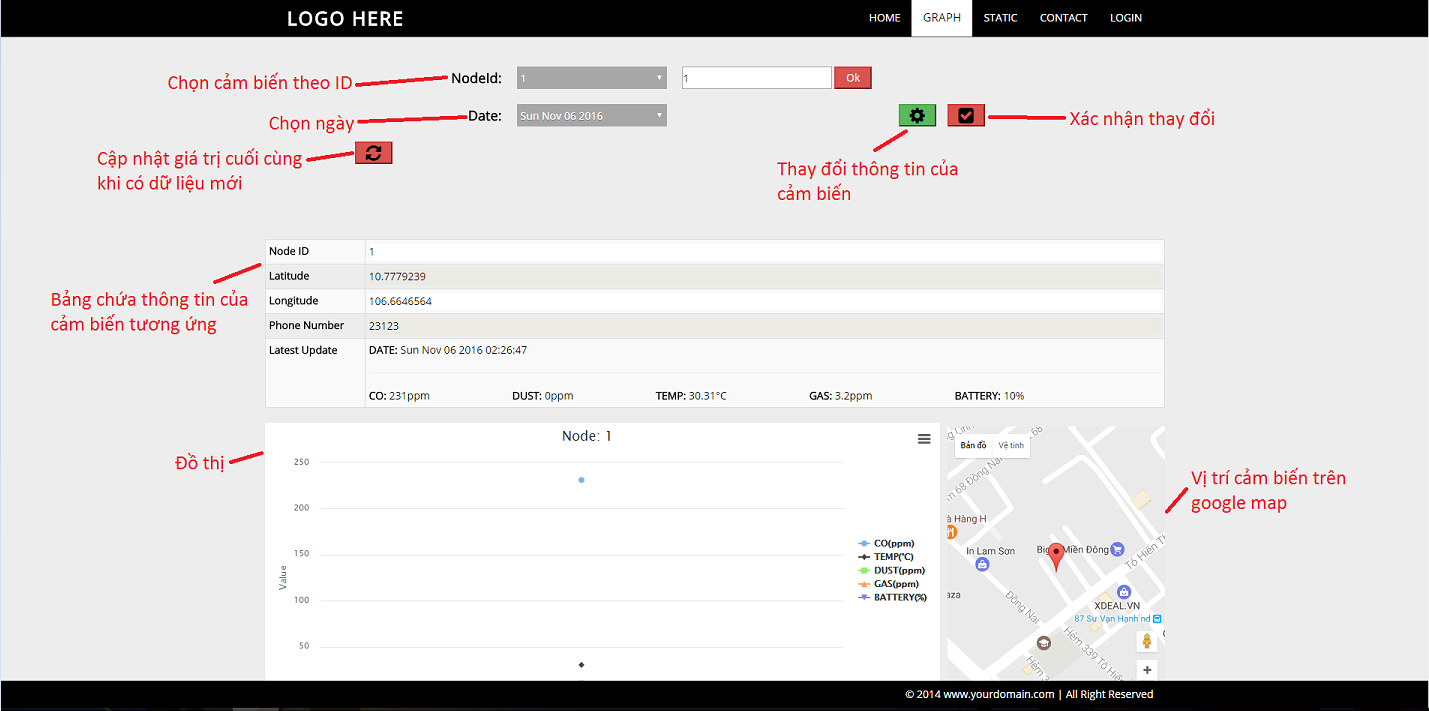
\includegraphics[width=1\textwidth]{web_graph}
		\caption[Giao diện đồ thị dữ liệu]{Giao diện đồ thị dữ liệu}
		\label{fig:web_graph}
	\end{figure}
\end{center}



\subsubsection*{Giao diện nhận feedback từ người dùng qua email}
Tương tác giữa người dùng với người quản lý server. Nội dung được gửi thông qua gmail.
\begin{center}
	\begin{figure}[H]
		\centering    
		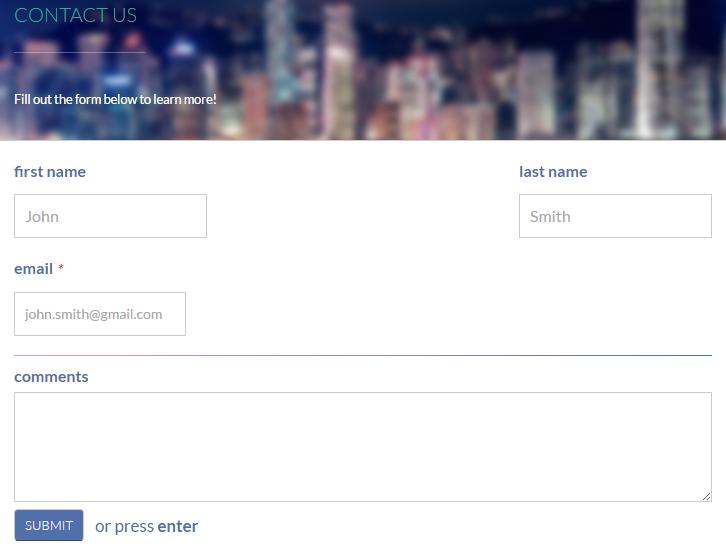
\includegraphics[width=1\textwidth]{web_email}
		\caption[Giao diện nhận feedback người dùng]{Giao diện nhận feedback người dùng}
		\label{fig:web_email}
	\end{figure}
\end{center}

\subsubsection*{Giao diện dành cho người quản lý}
Khu vực này dành cho người quản lý truy cập nhầm mục đích chỉnh sửa, thay thế các node cảm biến.
\begin{center}
	\begin{figure}[H]
		\centering    
		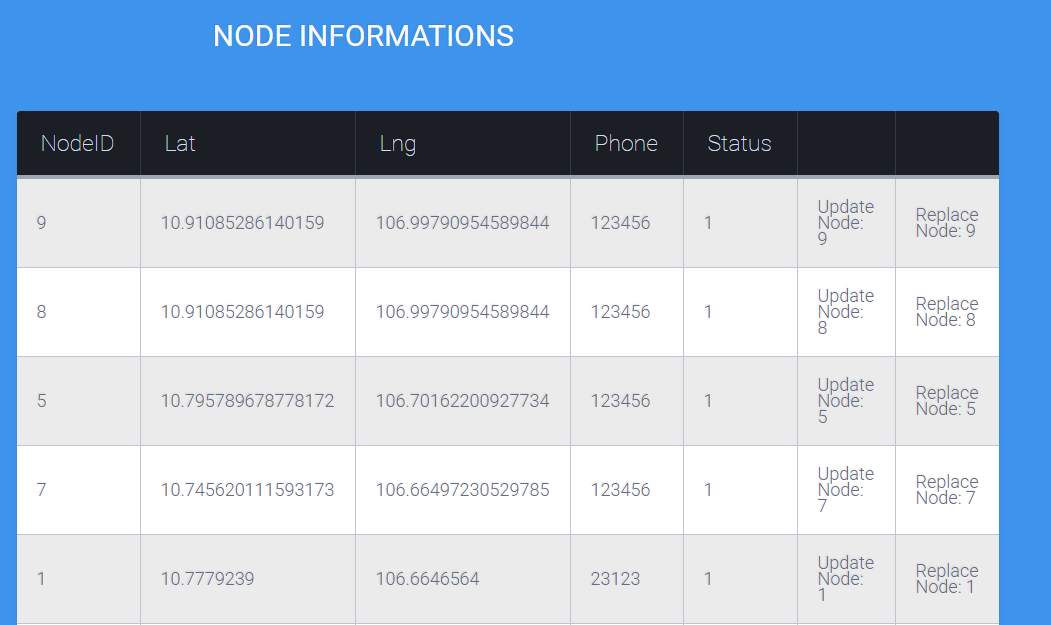
\includegraphics[width=1\textwidth]{web_nodeinfo}
		\caption[Giao diện quản lý các node cảm biến]{Giao diện quản lý các node cảm biến}
		\label{fig:web_nodeinfo}
	\end{figure}
\end{center}






\newpage
\section{Ứng dụng thiết bị di động}
\subsection{Hiện thực giao diện và chức năng}
\subsubsection*{Giao diện chính ứng dụng di động}
Tại giao diện chính của ứng dụng di động người dùng có thể xem được danh sách thông tin chi tiết của các node cảm biến có trong hệ thống.
\begin{figure}[H]
	\centering  
	\begin{subfigure}[b]{0.5\textwidth}
		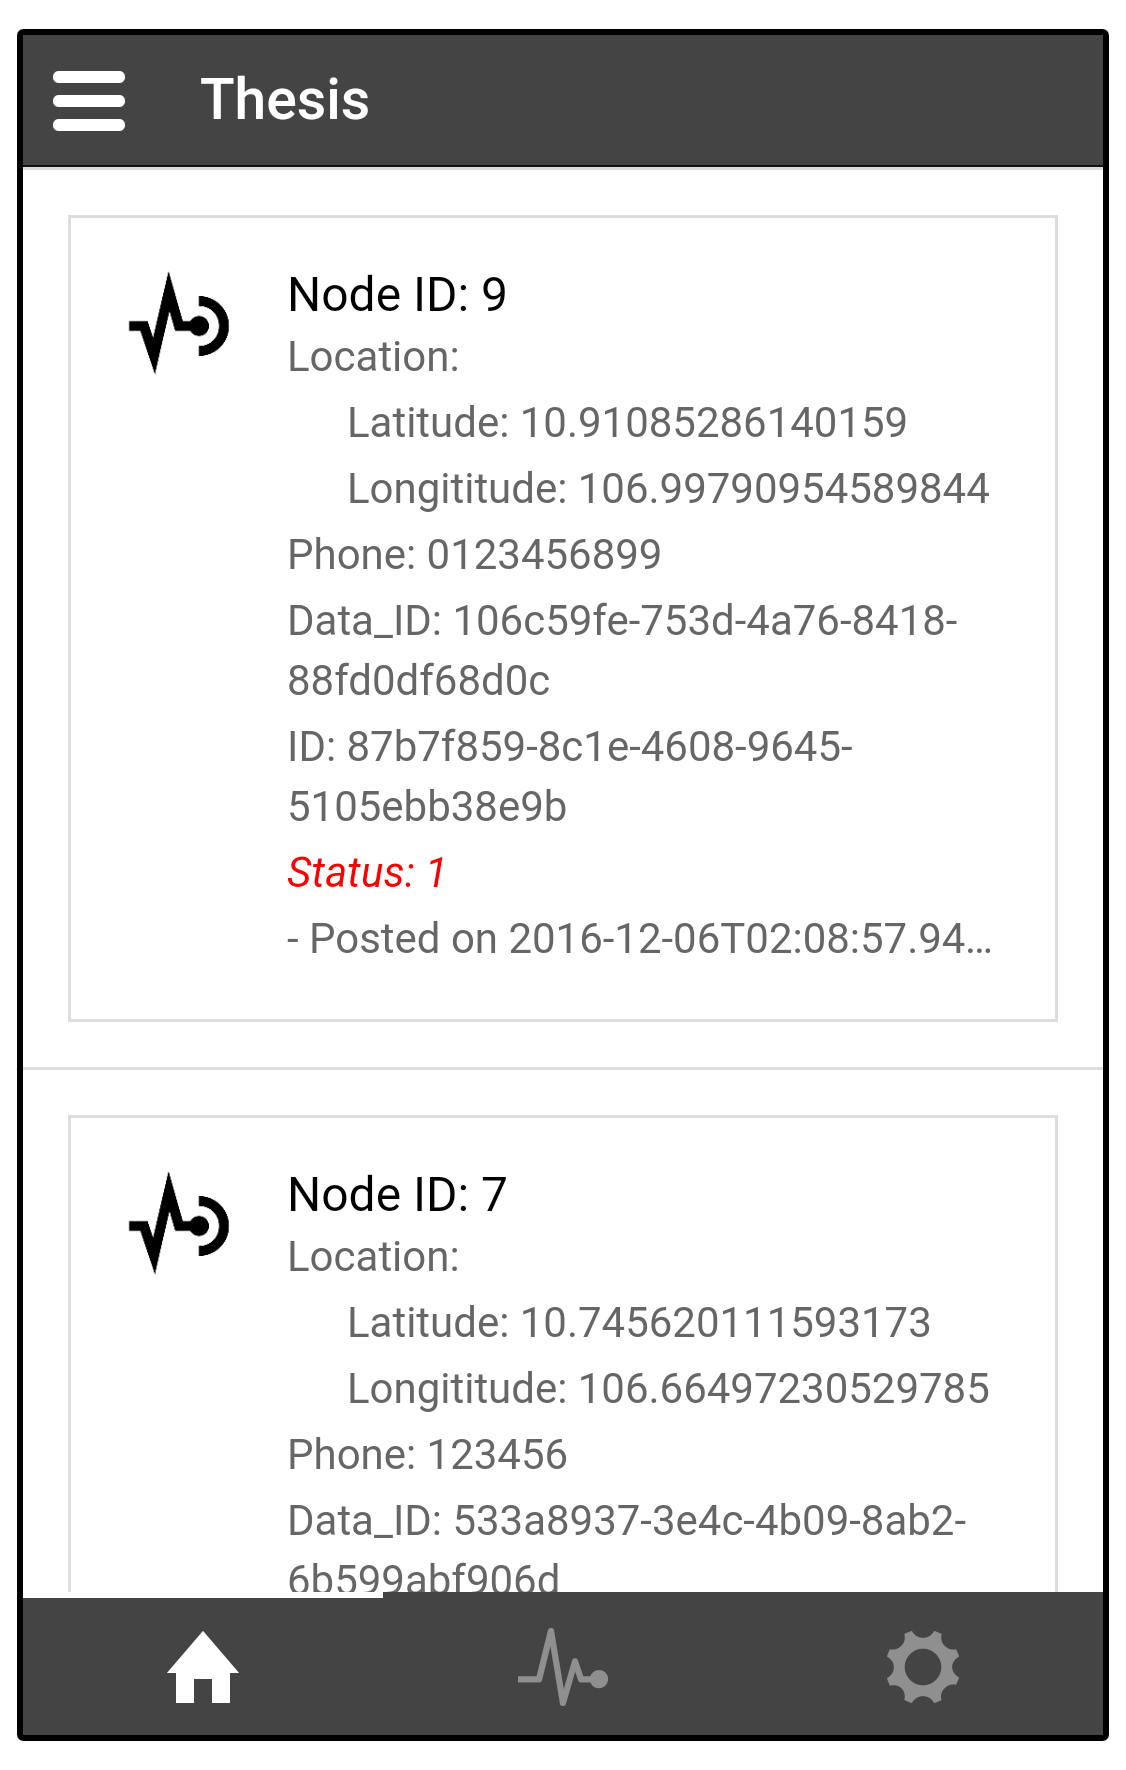
\includegraphics[width=2.5in]{main_1}
		\caption[Giao diện chính]{Giao diện chính}
		\label{fig:main_1}
	\end{subfigure}\hfill
	\begin{subfigure}[b]{0.5\textwidth}
		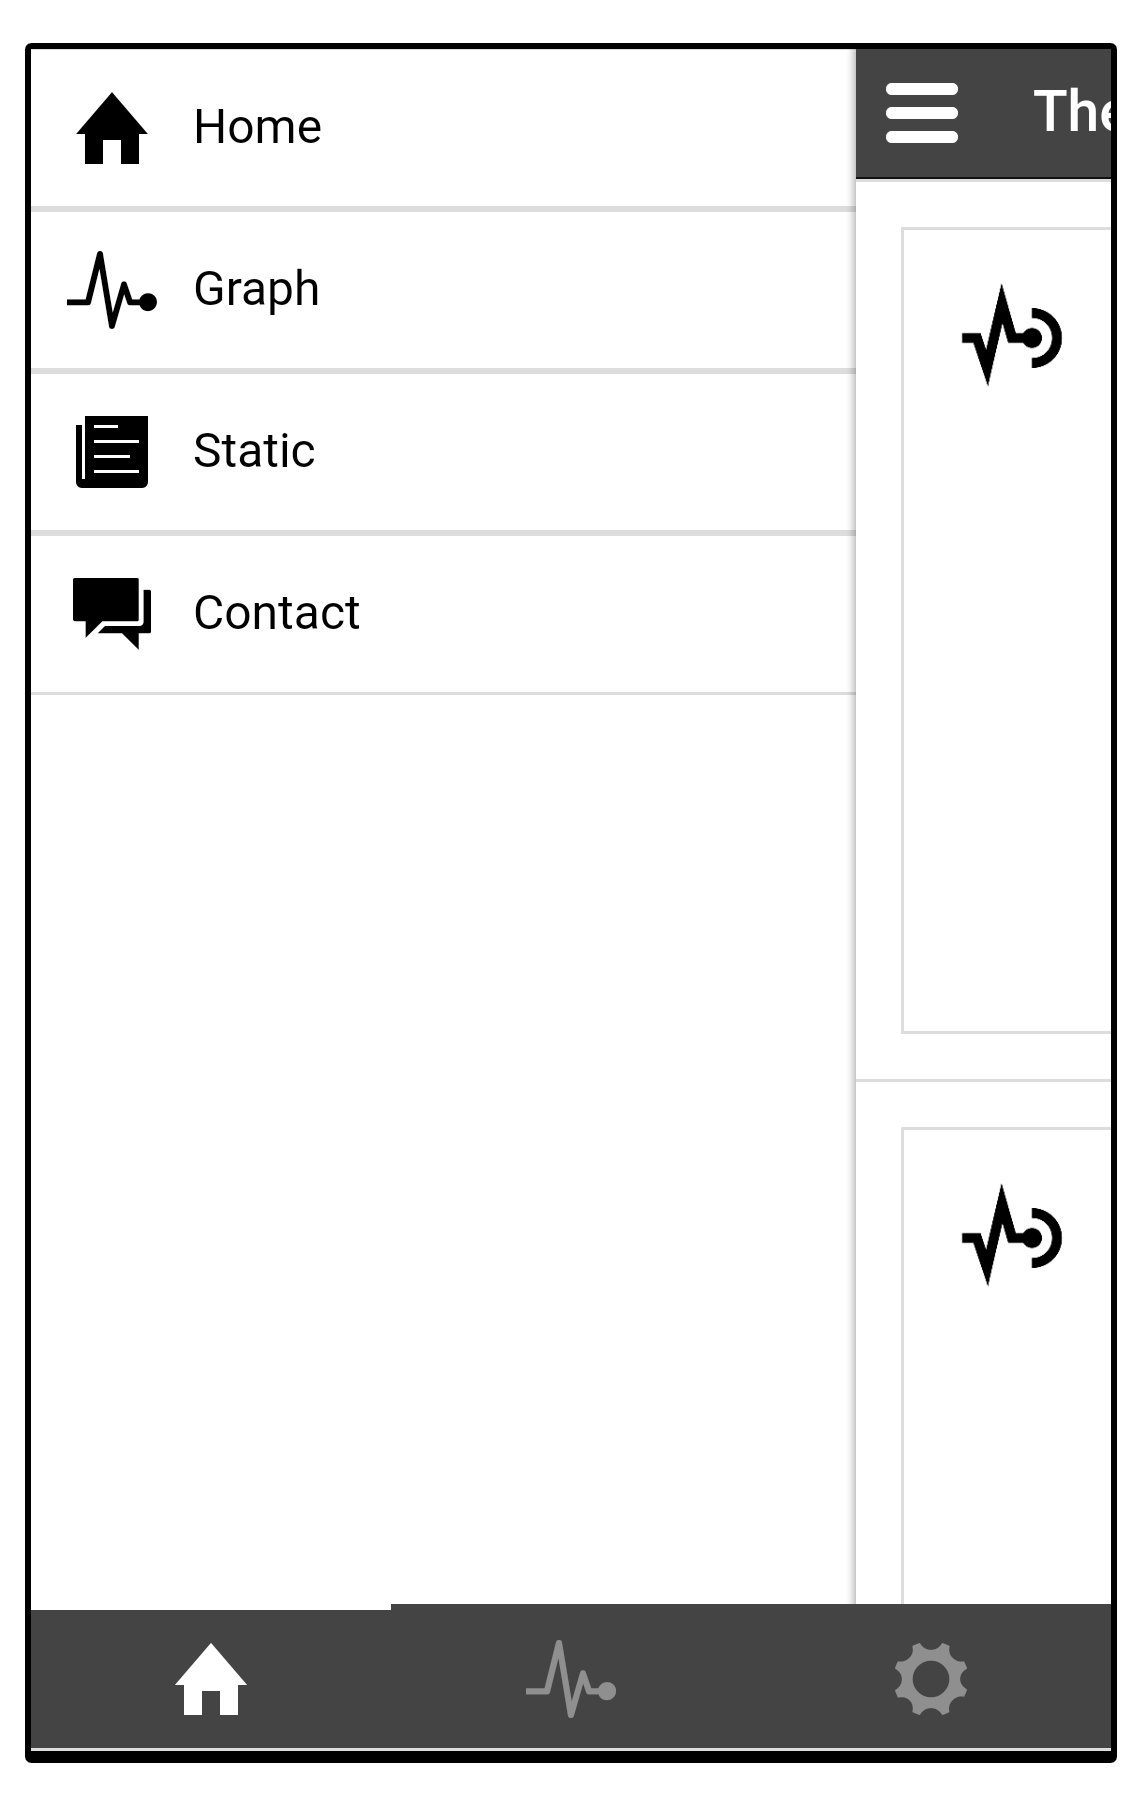
\includegraphics[width=2.5in]{main_2}
		\caption[Giao diện thanh menu]{Giao diện thanh menu}
		\label{fig:main_2}
	\end{subfigure}
	\caption{Giao diện chính ứng dụng di động}\label{fig:giaodienchinh}
\end{figure}


\subsubsection*{Giao diện xem dữ liệu trên ứng dụng di động}
Giao diện này cho phép người dùng theo dõi được dữ liệu của từng node cảm biến theo 2 loại biểu đồ như Hình \ref{fig:app_graph} thể hiện.
\begin{figure}[H]
	\centering  
	\begin{subfigure}[b]{0.5\textwidth}
		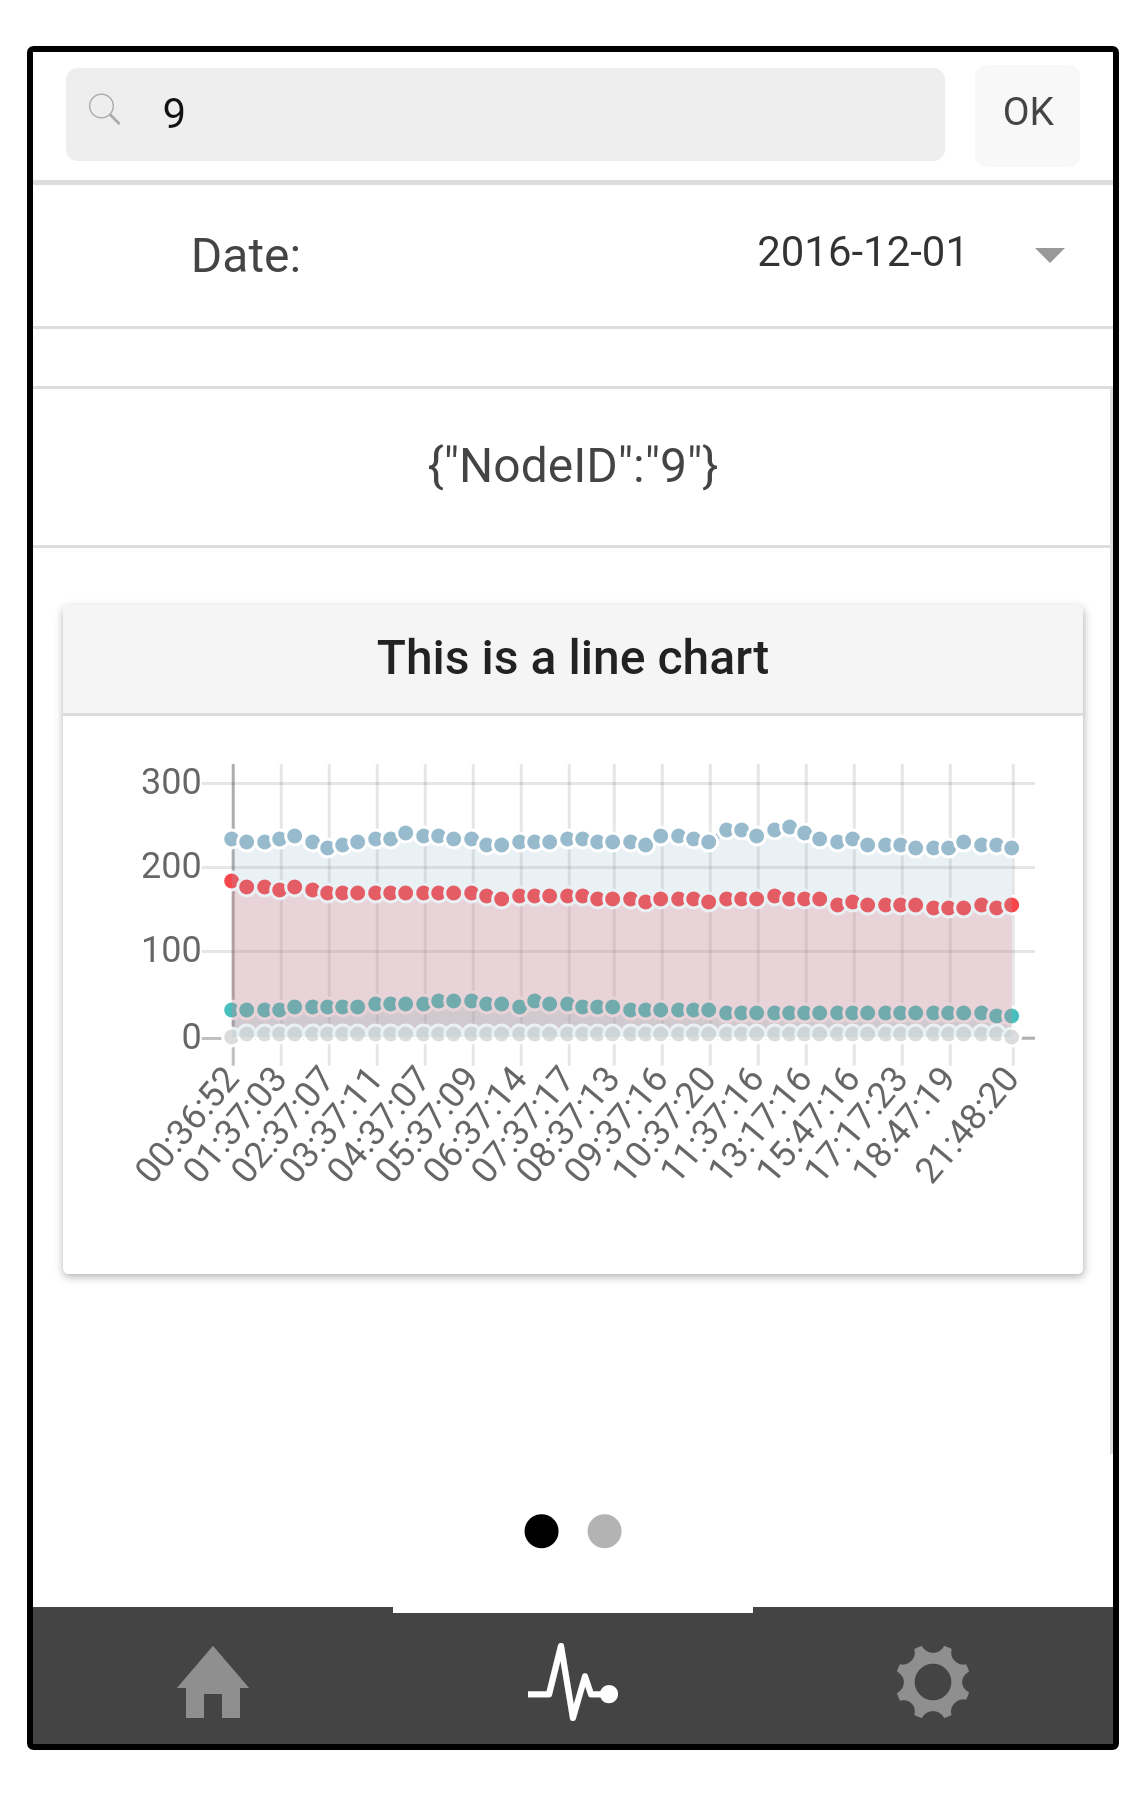
\includegraphics[width=2.5in]{main_4}
		\caption[Giao diện xem dữ liệu]{Giao diện xem dữ liệu}
		\label{fig:main_4}
	\end{subfigure}\hfill
	\begin{subfigure}[b]{0.5\textwidth}
		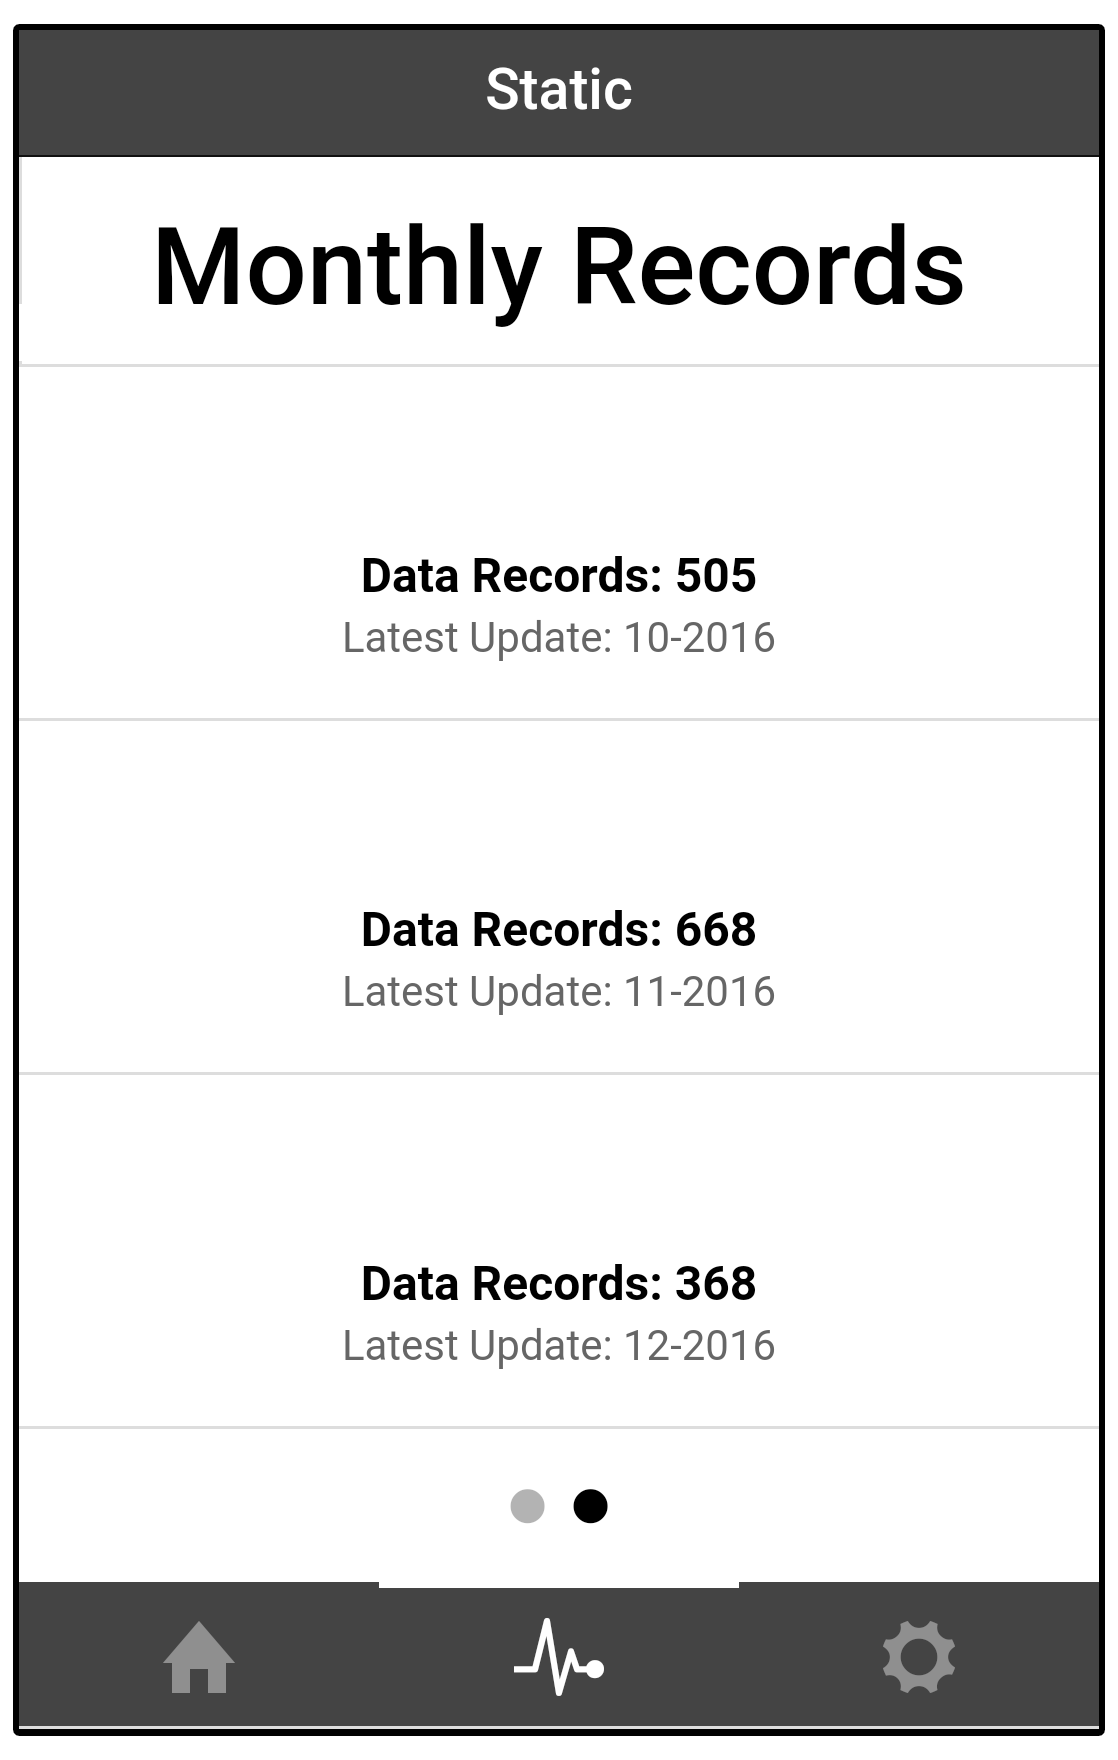
\includegraphics[width=2.5in]{main_3}
		\caption[Giao diện thống kê]{Giao diện thống kê}
		\label{fig:main_3}
	\end{subfigure}
	\caption{Giao diện ứng dụng di động}\label{fig:giaodienchinh2}
\end{figure}
\section{Tính ổn định của node cảm biến}
\textbf{này nói về mấy tháng đo, gió mưa đồ}

Lorem ipsum dolor sit amet, consectetur adipiscing elit, sed do eiusmod tempor incididunt ut labore et dolore magna aliqua. Ut enim ad minim veniam, quis nostrud exercitation ullamco laboris nisi ut aliquip ex ea commodo consequat. Duis aute irure dolor in reprehenderit in voluptate velit esse cillum dolore eu fugiat nulla pariatur. Excepteur sint occaecat cupidatat non proident, sunt in culpa qui officia deserunt mollit anim id est laborum
\section{Đánh giá Server}
\subsection{Tính sẵn sàng}
\begin{itemize}
\item[•] Hiện thực đoạn mã tự động khởi dộng Server khi nguồn điện có lại sau khi bị mất điện.\
\item[•] Sử dụng dịch vụ Dynamic DNS NOIP để cấu hình động tên miền gán với địa chỉ IP của Server tên miền hoạt động lại ngay sau khi vừa thay đổi địa chỉ IP(khắc phục sự cố mất điện làm IP thay đổi).
\end{itemize}
\subsection{Tính ổn định}
\begin{itemize}
	\item[•]Thực tế từ ngày khởi tạo Server và cho hoạt động liên tục 24/7 tới thời gian viết báo cáo là 8 tuần không có lỗi lạ xảy ra (trừ các trường hợp đặc biệt như mất điện, mạng mất kết nối)
	\item[•]Điện năng tiêu thụ thấp và nhiệt độ không quá cao, giao động (44 - 48 độ C) đảm bảo tốt trạng thái hoạt động.
\end{itemize}
\subsection{Tốc độ đáp ứng}
\begin{itemize}
	\item[•] Với sức mạnh của Raspberry Pi 3 thì Server hoạt đông tốt, thời gian tải file giao diện web nhanh với độ trễ thấp < 1s. Thời gian đáp ứng trung bình vào khoảng dưới 100ms là tải xong các tập tin giao diện web được gửi từ Server tới client.
	\item[•] Dịch vụ Google Maps hoạt động khá nhanh mặc dù gói tin truyền đi là chậm nhất vì lượng dữ liệu lớn.
	\item[•] API đáp ứng tốt, nhanh và hiệu quả. Thử nghiệm lập trình ứng dụng di động sử dụng API có thời gian đáp ứng tốt.
\end{itemize}

\section{Đánh giá lập trình ứng dụng Mobile sử dụng APIs}
\begin{itemize}
\item[•]Ứng dụng được viết có thể được xài trên nhiều platforms.
\item[•]Đã hiện thực được file APK cho mobile.
\item[•]Xây dựng một số các chức năng cơ bản như: hiện thị thông tin các node cảm biến cho màn hình chính, vẽ đồ thị, liên kết với web browser …
\item[•] Vẫn còn một vài chức năng cần hoàn thiện: đăng nhập quản lý người dùng, các chức năng phụ liên quan đến user …
\item[•] Khó khăn trong việc debugging vì một số plugin hay chức năng không chạy trên nền web app. 
\item[•]Hiệu suất thấp do nó không hoàn toàn tự nhiên, có thể gặp sự cố khi làm ứng dụng game hay các ứng dụng dùng nhiều tài nguyên.

\end{itemize}